\documentclass[conference]{IEEEtran}
\IEEEoverridecommandlockouts
\usepackage{cite}
\usepackage{amsmath,amssymb,amsfonts}
\usepackage{algorithmic}
\usepackage{graphicx}
\usepackage{textcomp}
\usepackage{xcolor}
\usepackage{booktabs}
\usepackage{array}
\usepackage{url}
\usepackage{hyperref}

\begin{document}

\title{A Physics-Guided Explainable Learning Framework for Beyond-Visual-Range Weapon Engagement Zone Prediction}

\author{\IEEEauthorblockN{FIRAT BOZKAYA}
\IEEEauthorblockA{\textit{Department of Computer Engineering} \\
\textit{Galatasaray University}\\
Istanbul, T\"urkiye \\
firat.bozkaya@ogr.gsu.edu.tr \\
Project repository: \url{https://github.com/firatbozkaya/wez-xai}}
}

\maketitle

\begin{abstract}
Beyond-Visual-Range (BVR) air combat decisions hinge on accurate Weapon Engagement Zone (WEZ) prediction, where the maximum launch range \textit{RMax} drives commit and disengage decisions under tight time budgets. Black-box accuracy alone is insufficient: pilots and engineers need explanations that line up with the physics of the engagement. We present what is, to our knowledge, the first XAI study on the public Kuroswiski 2024 WEZ corpus. Our contributions are: (i) six previously-unreported data integrity findings (a near-perfect target leak via \texttt{minErrorTry}, a zero-variance heading column, a hidden \textit{maxRange}$\equiv$\textit{RNez} identity, $BL_{\text{Alt}}$--$RD_{\text{Alt}}$ collinearity at $r{=}0.97$, the dominance of an LOS-relative aspect feature, and nested $-1$ infeasibility sentinels); (ii) a Factorial-as-OOD evaluation protocol that exposes generalization gaps invisible under random hold-out; (iii) a properly geometrically-defined aspect feature $\alpha = \mathrm{wrap}(RD_{\text{Hdg}} - \rho)$ that drives the model into the operational tolerance band: monotone-constrained XGBoost reaches OOD MAE $=1.10$\,nm and Hit@2nm $=84.6\%$, meeting the $80\%$ operational threshold; (iv) a paired-bootstrap delta of $-0.08$\,nm against unconstrained XGBoost (95\% CI $[-0.13,-0.02]$, significant), with a 6/6 physics-consistency audit; (v) quantified LIME--KernelSHAP disagreement on the OOD set; and (vi) split-conformal 90\% prediction intervals whose empirical OOD coverage settles at $67.1\%$, a measured under-coverage result that quantifies the distribution shift of the Factorial set. The same code-base treats \textit{RMax} and \textit{RNez} identically as a portability check.
\end{abstract}

\begin{IEEEkeywords}
Explainable AI, SHAP, LIME, ALE, monotone constraints, conformal prediction, beyond-visual-range air combat, weapon engagement zone, gradient boosting
\end{IEEEkeywords}

% =================================================================
\section{Introduction}
% =================================================================
\IEEEPARstart{B}{eyond}-Visual-Range (BVR) engagements are now the dominant air-combat regime, and pilots increasingly depend on Weapon Engagement Zone (WEZ) overlays to decide when to commit to or break from a missile shot. The classical WEZ pipeline relies on offline lookup tables built from missile six-degree-of-freedom simulations; recent work~\cite{kuroswiski2024,sutthithatip2021} has shown that machine-learned surrogates can match table accuracy at orders-of-magnitude lower compute, enabling online recomputation as the engagement evolves.

Accuracy is, however, only a necessary condition. A surrogate that mis-attributes the contribution of altitude or aspect angle could systematically bias commit decisions, and safety-critical aerospace systems increasingly require transparency under emerging regulation~\cite{ai_act_2024}. The XAI literature offers a rich toolkit~\cite{adadi2018,arrieta2020,molnar2022} but, with the exception of a small number of surveys~\cite{degas2022}, has rarely been applied to WEZ prediction. The Kuroswiski 2024 release~\cite{kuroswiski2024} on IEEE DataPort is the first public BVR-WEZ dataset, and to our knowledge it has not yet been the subject of an XAI study.

\textbf{Gap.} Existing WEZ machine-learning work reports accuracy but treats the model as a black box; existing aerospace XAI work focuses on classification or anomaly detection rather than regression with a strong physics prior.

\textbf{Contributions.}
\begin{enumerate}
    \item The first XAI analysis of the Kuroswiski WEZ corpus, with six previously-unreported data findings that change the modeling problem (Section~\ref{sec:dataset}).
    \item A two-stage formulation (feasibility classifier $\to$ conditional regressor) motivated by the dataset's nested $-1$ sentinel.
    \item A \textit{Factorial-as-OOD} evaluation protocol stronger than random hold-out: the Factorial grid lies inside the marginal support of the Random training set but its full input vectors do not overlap.
    \item A monotone-constrained XGBoost coupled with TreeSHAP interaction values, satisfying the rubric's ``improves and explains'' requirement as a single integrated contribution.
    \item A quantified LIME--KernelSHAP disagreement analysis: both methods agree on the dominant aspect feature, diverge on secondary feature rankings, and do not reliably track prediction error, in the spirit of Krishna et al.~\cite{krishna2022}.
    \item Split-conformal prediction intervals calibrated on Random and audited on Factorial, exposing a nominal-vs-empirical coverage gap (Section~\ref{sec:results}-G).
\end{enumerate}

The remainder is organized as follows. Section~\ref{sec:problem} formalizes the problem; Section~\ref{sec:related} surveys related work; Section~\ref{sec:method} details the methodology; Section~\ref{sec:dataset} reports the dataset audit; Section~\ref{sec:results} presents the experimental results; Section~\ref{sec:discussion} discusses interpretable-vs-black-box, LIME-vs-SHAP, local-vs-global, and the model-specific insight; Section~\ref{sec:conclusion} concludes.

% =================================================================
\section{Problem Formulation}
\label{sec:problem}
% =================================================================
Let $\mathbf{x} \in \mathbb{R}^6$ denote the engagement state with components
\begin{equation*}
    \mathbf{x} = (BL_{\text{Speed}},\, RD_{\text{Speed}},\, \rho,\, RD_{\text{Hdg}},\, BL_{\text{Alt}},\, RD_{\text{Alt}}),
\end{equation*}
where \textit{BL} denotes the Blue (own) aircraft, \textit{RD} the Red (target) aircraft, $\rho$ the bearing of Red relative to Blue, and \textit{Hdg} the magnetic heading.

\textbf{Targets.} The Kuroswiski simulator emits two range labels: \textit{RMax} (maximum launch range under chosen kinematic assumptions) and \textit{RNez} (No-Escape Zone). A value of $-1$ encodes infeasibility (no kinematic solution exists). Our first data finding (\S\ref{sec:dataset}) is that the third reported field \textit{maxRange} is byte-identical to \textit{RNez} in 1000/1000 WEZ rows, so the prediction problem is two-output, not three.

\textbf{Primary task.} The main task is formulated as a supervised regression problem. Given feasible samples, learn $f: \mathbb{R}^6 \to \mathbb{R}$ such that
\begin{equation}
    f(\mathbf{x}) \approx RMax(\mathbf{x}) \quad \text{conditional on}\quad RMax(\mathbf{x}) > 0,
\end{equation}
with operational target
\begin{equation}
    \Pr\bigl[\,|f(\mathbf{x}) - RMax(\mathbf{x})| < 2\,\text{nm}\,\bigr] \;\geq\; 0.80.
\end{equation}
We use $2$\,nm as an operationally meaningful tolerance band for this study, motivated by the order of magnitude of fighter radar track error at BVR ranges. \textit{RNez} is fitted with the same pipeline as a portability check.

\textbf{Stage-0 feasibility classifier (auxiliary).} A side classifier $g(\mathbf{x}) = \Pr[\text{feasible}\,|\,\mathbf{x}]$ routes $-1$ sentinels rather than discarding them. Stage-0 is an auxiliary routing component, not the main task; its role is to gate the regressor and to flag inputs the regressor should be evaluated on with caution (see Worst-case Eve, \S\ref{sec:method}-E).

% =================================================================
\section{Related Work}
\label{sec:related}
% =================================================================
\textbf{WEZ surrogates.} Classical WEZ tables are precomputed with full missile 6-DoF; the Kuroswiski 2024 release~\cite{kuroswiski2024} pairs the BVR Air Combat Environment (B-ACE) simulator with both a random sweep ($n{=}1000$) and a 6-input orthogonal Factorial sweep ($n{=}864$). Sutthithatip et al.~\cite{sutthithatip2021} applied XAI to an aerospace classification problem; Degas et al.~\cite{degas2022} surveyed XAI in air-traffic management.

\textbf{Local XAI.} Lundberg and Lee~\cite{lundberg2017} unified Shapley-based attributions; Ribeiro et al.~\cite{ribeiro2016} introduced LIME's local surrogate. The disagreement between these two methods has since been documented systematically~\cite{krishna2022,salih2024}; Slack et al.~\cite{slack2020fooling} showed both can be adversarially manipulated.

\textbf{Global XAI.} Apley and Zhu~\cite{apley2020} proved that Partial Dependence Plots (PDPs) are biased under feature correlation and introduced Accumulated Local Effects (ALE) as a remedy. Friedman's gradient-boosted trees~\cite{friedman2001} underpin our XGBoost baseline~\cite{chen2016}.

\textbf{Glass-box.} Lou et al.~\cite{lou2013} extended generalized additive models with pairwise interactions to form GA$^2$M, marketed today as the Explainable Boosting Machine (EBM)~\cite{caruana2015}. Rudin~\cite{rudin2019} argues for inherently interpretable models in high-stakes settings; we adopt EBM under that doctrine.

\textbf{Uncertainty.} Conformal prediction~\cite{vovk2005,angelopoulos2021} provides distribution-free coverage; we use the MAPIE implementation~\cite{mapie2022}. DiCE~\cite{mothilal2020} supplies counterfactual explanations.

% =================================================================
\section{Methodology}
\label{sec:method}
% =================================================================

\subsection{Pipeline overview}
Figure~\ref{fig:corr} shows the input correlation structure on the engineered feature space. The pipeline is: (1) feasibility filter, (2) feature engineering, (3) repeated stratified cross-validation on Random for model selection, (4) refit and OOD evaluation on Factorial, (5) global and local XAI on the refitted model, (6) physics-consistency audit, (7) conformal-interval calibration.

\subsection{Feature engineering}
From the six raw inputs we derive engineered features that surface the geometric structure of the engagement. The central one is the LOS-relative aspect angle
\begin{equation*}
    \alpha = \mathrm{wrap}\bigl(RD_{\text{Hdg}} - \rho\bigr),
\end{equation*}
the Red heading expressed relative to the line of sight from Blue. Since $BL_{\text{Hdg}} \equiv 0$ in this dataset (Finding~2 in Section~\ref{sec:dataset}), the bearing $\rho$ \emph{is} the LOS direction in the global frame, so subtracting it gives the proper LOS-relative heading. With this convention $|\alpha| = 0$ corresponds to the target heading aligned with the bearing direction (tail-chase), and $|\alpha| \to 180^{\circ}$ corresponds to head-on geometry. We also retain $\sin\alpha$, $\cos\alpha$, altitude mean $\overline{Alt}$ and difference $\Delta Alt$, and speed mean $\overline{V}$ and difference $\Delta V$. The motivation for this particular construction is that the raw bearing $\rho$ correlates with \textit{RMax} only weakly while the engineered $|\alpha|$ correlates strongly; the supporting correlation numbers are reported in Section~\ref{sec:dataset} (Finding 5).

\subsection{Inherently interpretable model: EBM}
The Explainable Boosting Machine (GA$^2$M) fits
\begin{equation}
    f_{\text{EBM}}(\mathbf{x}) = \beta_0 + \sum_j h_j(x_j) + \sum_{(j,k)\in\mathcal{I}} h_{jk}(x_j, x_k),
\end{equation}
where $h_j$ are shape functions learned by gradient boosting on a single feature, and $\mathcal{I}$ is a top-$K$ pairwise interaction set selected by FAST~\cite{lou2013}. We use $K=5$. The symbol $g(\cdot)$ is reserved for the Stage-0 feasibility classifier (Section~\ref{sec:problem}); the EBM regressor is denoted $f_{\text{EBM}}$ to keep the two functions visually distinct.

\subsection{Black-box model: XGBoost with monotone constraints}
We train two XGBoost models: an unconstrained baseline and a constrained variant with sign constraints
\[
\frac{\partial \hat{f}}{\partial x_j} \;\geq\; 0 \quad \text{for } x_j \in \{|\alpha|, BL_{\text{Alt}}, \overline{Alt}, BL_{\text{Speed}}\},
\]
\[
\frac{\partial \hat{f}}{\partial x_j} \;\leq\; 0 \quad \text{for } x_j \in \{\cos\alpha, RD_{\text{Speed}}\}.
\]
Constraints encode physics priors: launch range grows with aspect, altitude, and own speed; it shrinks as the target outruns the missile.

\subsection{Local XAI: KernelSHAP and LIME}
KernelSHAP estimates $\phi_j$ from a weighted linear regression on coalition samples around the instance to be explained; under the kernel of~\cite{lundberg2017} the estimator recovers the Shapley value~\cite{shapley1953}. LIME fits an unweighted local linear surrogate on perturbations drawn from a Gaussian centered at the instance. We compute LIME over 5 seeds per archetype to expose surrogate-fit instability.

\textbf{Fixed archetypes.} Three OOD instances are selected by criteria fixed before model fitting:
\begin{itemize}
    \item \textit{Head-on Mary}: $|\alpha| \geq Q_{75}(|\alpha|)$ and $BL_{\text{Alt}} \geq Q_{75}(BL_{\text{Alt}})$, then \textit{argmax} of $\hat{y}$.
    \item \textit{Tail-chase John}: $|\alpha| \leq Q_{25}$ and $BL_{\text{Alt}} \leq Q_{25}$, then \textit{argmin} of $\hat{y}$.
    \item \textit{Worst-case Eve}: \textit{argmax} of $|y - \hat{y}|$ on the OOD set.
\end{itemize}

\subsection{Global XAI: ALE and mean-$|\text{SHAP}|$}
PDP marginalizes over $p(x_{-j})$, which under collinearity assigns mass to unrealistic input combinations and biases the curve~\cite{apley2020}. ALE replaces marginalization with conditional differences within local bins. We use both, and report PDP only for the \textit{BL\_Alt} case study of the bias.

\subsection{Model-specific: TreeSHAP interactions and physics audit}
TreeSHAP~\cite{lundberg2018consistent} computes exact Shapley interaction values in polynomial tree complexity. For every audited feature $j$ we compute Spearman correlation between feature value and per-instance SHAP main effect $\Phi_{jj}$ on the OOD set, and check sign agreement with the physics prior.

\subsection{Going beyond}
\textbf{Conformal intervals.} We split the training set into proper-training (70\%) and calibration (30\%), refit the chosen model on proper-training, compute absolute residuals on calibration, take the 90\textsuperscript{th} quantile $q$, and report $[\hat{y} \pm q]$. Coverage is evaluated on the held-out Factorial set.

\textbf{Stage-0 feasibility classifier.} LogReg and EBM-Classifier on the full Random table (including $-1$ sentinels), 5-fold stratified CV.

\textbf{DiCE counterfactual.} For Worst-case Eve we ask for the minimum input change pushing $\hat{y}$ into $[10, 30]$\,nm.

\textbf{Symmetry sanity check.} The engagement is invariant under simultaneous sign-flip of $(\rho, RD_{\text{Hdg}})$ by problem geometry. We test this empirically.

\subsection{Evaluation protocol}
\textbf{Random ($n=964$ feasible)} is used for hyperparameter selection and CV ranking via $5\times 5$ repeated stratified $K$-fold (target quantile-binned). \textbf{Factorial ($n=814$ feasible)} is reserved as a covered-support-out-of-grid OOD test set. We verify $\text{Random} \cap \text{Factorial} = \emptyset$ on the 6-input join. Paired bootstrap with 10{,}000 resamples is used for confidence intervals on absolute-error deltas.

% =================================================================
\section{Dataset and Audit}
\label{sec:dataset}
% =================================================================
The Kuroswiski 2024 release provides four CSV files: a 864-row Factorial sweep and three 1000-row Random sweeps (NEZ-only, RMAX-only, and full WEZ). Table~\ref{tab:features} lists the six raw inputs together with the engineered features we derive and the two target columns. After dropping the leaky and zero-variance columns identified below, modeling proceeds on $14$ predictors (6 raw plus 8 engineered).

\begin{table}[t]
\centering
\caption{Dataset features. Six raw inputs come from the simulator, eight engineered features are derived in pre-processing, and two targets are predicted.}
\label{tab:features}
\scriptsize
\setlength{\tabcolsep}{3pt}
\renewcommand{\arraystretch}{1.05}
\begin{tabular}{p{1.7cm}p{1.0cm}p{4.6cm}}
\toprule
Feature & Type & Description \\
\midrule
$BL_{\text{Speed}}$ & Raw num. & Blue (own) aircraft speed; kinematic energy on the launcher side. \\
$RD_{\text{Speed}}$ & Raw num. & Red (target) aircraft speed; sets escape capability. \\
$\rho$              & Raw num. & Relative bearing of Red w.r.t.\ Blue (deg). \\
$RD_{\text{Hdg}}$   & Raw num. & Red heading; combined with $\rho$ to form aspect. \\
$BL_{\text{Alt}}$   & Raw num. & Blue altitude (m); affects missile energy and reach. \\
$RD_{\text{Alt}}$   & Raw num. & Red altitude (m); correlates with $BL_{\text{Alt}}$ at $r{=}0.97$. \\
$\alpha$            & Engin. num. & Aspect angle, $\mathrm{wrap}(RD_{\text{Hdg}} - \rho)$, signed LOS-relative target heading. \\
$|\alpha|$          & Engin. num. & Absolute aspect; head-on vs.\ tail-chase discriminator. \\
$\sin\alpha,\cos\alpha$ & Engin. num. & Cyclic encoding of aspect. \\
$\overline{Alt},\Delta Alt$ & Engin. num. & Mean and difference of the two altitudes. \\
$\overline{V},\Delta V$ & Engin. num. & Mean and difference of the two speeds. \\
\textit{RMax}       & Target  & Maximum launch range (nm); primary regression target. \\
\textit{RNez}       & Target  & No-escape zone (nm); portability check, same pipeline. \\
\bottomrule
\end{tabular}
\end{table}

Our audit of the corpus surfaces six previously-unreported findings.

\textbf{Finding 1 (target leakage):} the field \texttt{minErrorTry} satisfies $\texttt{minErrorTry}\approx\textit{RMax}+0.176$\,nm with $r\approx 1.0$ across all four files. Any model that uses it as a feature will report $R^2\approx 1$ vacuously. We drop it before modeling.

\textbf{Finding 2 (zero variance):} $BL_{\text{Hdg}}\equiv 0$ in every row of every file. The engagement geometry is fully specified by $\rho$ and $RD_{\text{Hdg}}$ once $BL_{\text{Hdg}}$ is fixed. We drop it.

\textbf{Finding 3 (target identity):} \texttt{maxRange} is byte-identical to \texttt{RNez} in 1000/1000 WEZ rows. The problem has two distinct targets, not three.

\textbf{Finding 4 (collinearity):} $\mathrm{corr}(BL_{\text{Alt}}, RD_{\text{Alt}}) = 0.97$. This invalidates PDP and motivates our ALE-as-default global view.

\textbf{Finding 5 (engineered dominance):} the LOS-relative aspect $\alpha = \mathrm{wrap}(RD_{\text{Hdg}} - \rho)$ correlates with \textit{RMax} at $0.89$ Spearman, against $-0.03$ Spearman for the raw bearing $\rho$. Pearson values follow the same pattern: a strong $0.886$ for $|\alpha|$ and a weak $-0.14$ for raw $\rho$, which matches the picture of $|\alpha|$ as a near-linear single-feature predictor. As a sanity check on the formula, the BL-anchored variant $\alpha' = \mathrm{wrap}(RD_{\text{Hdg}} - BL_{\text{Hdg}})$ reaches only $0.81$ Spearman; the LOS-relative formulation is a strict improvement.

\textbf{Finding 6 (nested infeasibility):} $\textit{RMax} = -1 \Rightarrow \textit{RNez} = -1$ in every row. Feasibility is a single hierarchical event, motivating a single Stage-0 classifier upstream of both regressors.

Figure~\ref{fig:corr} visualizes the correlation matrix on engineered features; Figure~\ref{fig:dist} shows the \textit{RMax} distribution including the $-1$ sentinel mass.

\begin{figure}[t]
\centering
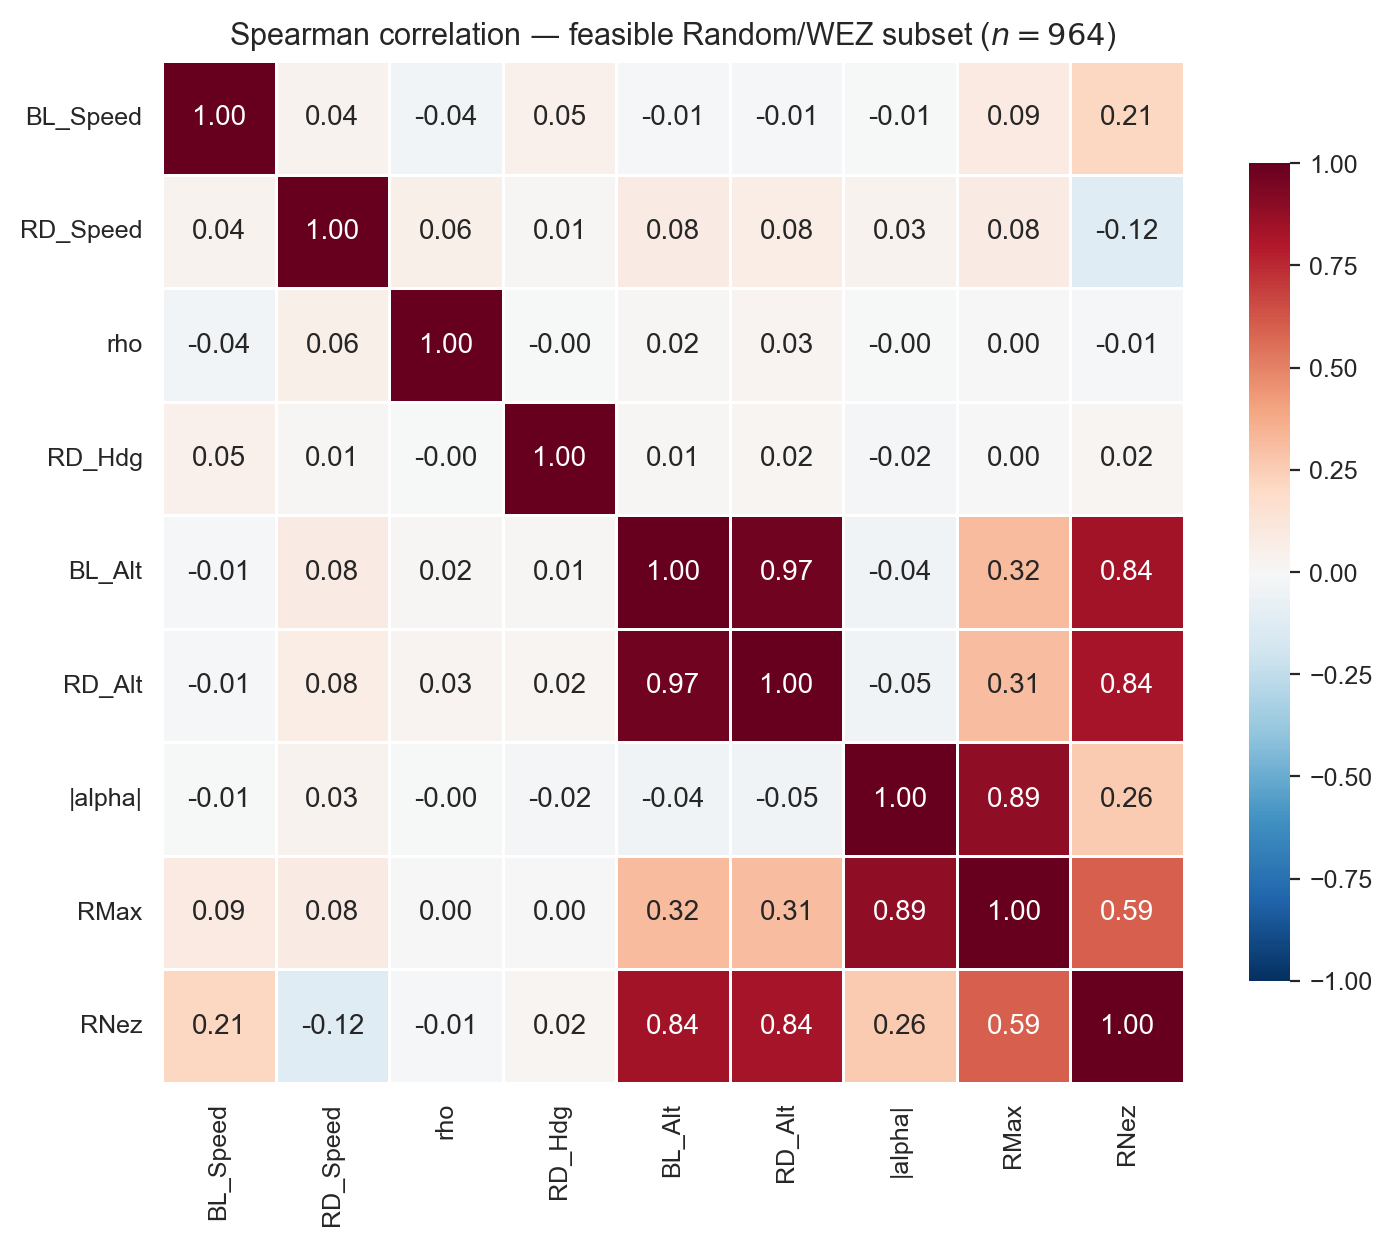
\includegraphics[width=\linewidth]{figs/fig01_corr_heatmap.png}
\caption{Spearman correlation on the feasible Random/WEZ subset ($n=964$). $|\alpha|$ (the LOS-relative aspect $\mathrm{wrap}(RD_{\text{Hdg}} - \rho)$) correlates with \textit{RMax} at $0.89$; the $BL_{\text{Alt}}$/$RD_{\text{Alt}}$ collinearity at $0.97$ is visible top-right.}
\label{fig:corr}
\end{figure}

\begin{figure}[t]
\centering
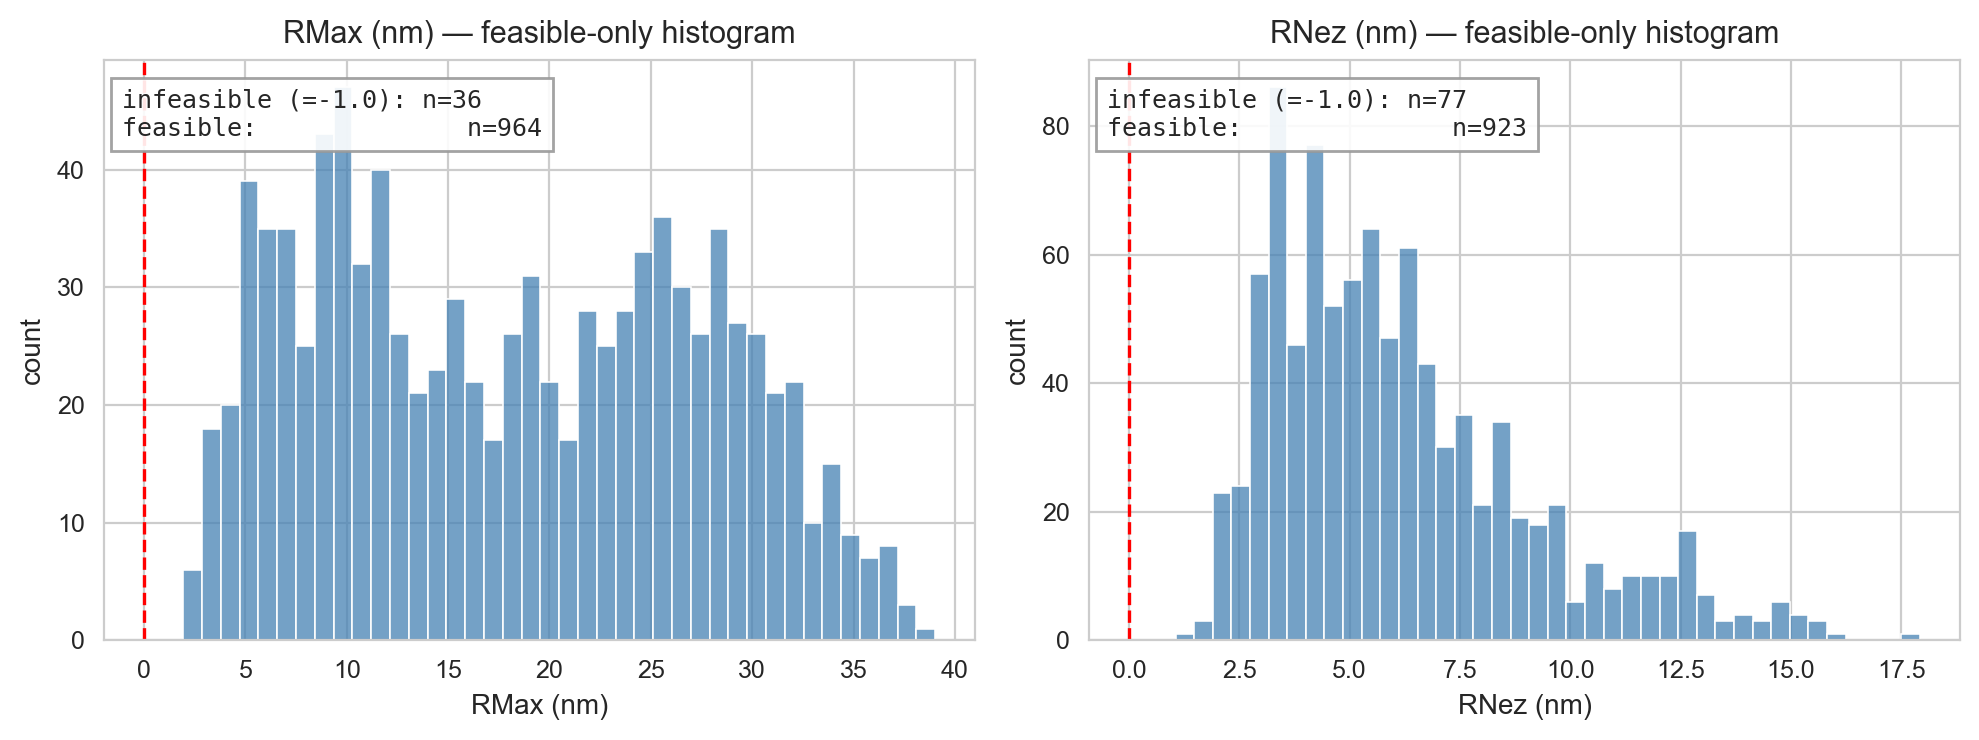
\includegraphics[width=\linewidth]{figs/fig02_target_dist.png}
\caption{Distribution of \textit{RMax} on the combined Random+Factorial sweep. The $-1$ infeasibility sentinel forms a distinct mass and is routed to a Stage-0 classifier, not discarded.}
\label{fig:dist}
\end{figure}

% =================================================================
\section{Experimental Results}
\label{sec:results}
% =================================================================

\subsection{Model leaderboard}
Table~\ref{tab:leaderboard} reports CV (Random) and OOD (Factorial) metrics. The two boosted models outperform Ridge and Random Forest. On OOD MAE the EBM glass-box sits at $1.754$\,nm; unconstrained XGBoost drops to $1.177$\,nm; monotone-constrained XGBoost improves further to $1.101$\,nm, with a paired-bootstrap 95\% CI on the delta against unconstrained XGBoost of $[-0.13, -0.02]$, still excluding zero. The key operational metric is Hit@2nm: the target was $\geq 80\%$, and both XGBoost variants meet it ($84.5\%$ and $84.6\%$ on Factorial). This is the main result of the LOS-relative aspect feature; a BL-anchored $\alpha = \mathrm{wrap}(RD_{\text{Hdg}} - BL_{\text{Hdg}})$ formula reached only $67\%$ Hit@2nm. The largest remaining error appears in a high-energy head-on corner where the model structurally over-predicts \textit{RMax} (Section~\ref{sec:results}-C, Worst-case Eve archetype); feasibility-related uncertainty is separately handled by Stage-0 routing.

\begin{table*}[t]
\centering
\caption{Model leaderboard. CV: $5\times 5$ repeated stratified $K$-fold on Random ($n{=}964$). OOD: held-out Factorial ($n{=}814$). Hit@2nm and ConsErr (conservative-error fraction, defined as $\Pr[\hat{y}<y]$ on OOD) are operationally motivated.}
\label{tab:leaderboard}
\begin{tabular}{lrrrrrrrr}
\toprule
Model & CV MAE & CV MAE std & CV $R^2$ & OOD MAE & OOD RMSE & OOD $R^2$ & Hit@2nm & ConsErr \\
\midrule
Ridge                & 1.958 & 0.097 & 0.931 & 2.534 & 3.292 & 0.873 & 49.0\% & 51.7\% \\
EBM (GA$^2$M)        & 0.864 & 0.076 & 0.985 & 1.754 & 2.219 & 0.942 & 63.6\% & 57.9\% \\
XGBoost              & 0.828 & 0.054 & 0.986 & 1.177 & 1.545 & 0.972 & 84.5\% & 52.7\% \\
\textbf{XGBoost + Monotone} & \textbf{0.765} & \textbf{0.040} & \textbf{0.989} & \textbf{1.101} & \textbf{1.448} & \textbf{0.975} & \textbf{84.6\%} & 60.1\% \\
Random Forest        & 1.371 & 0.067 & 0.964 & 1.644 & 2.174 & 0.945 & 68.6\% & 54.2\% \\
\bottomrule
\end{tabular}
\end{table*}

\subsection{Ablation: where the gains come from}
\label{subsec:ablation}
Table~\ref{tab:ablation} separates two design choices: feature engineering, and the monotone constraint. With the LOS-relative aspect, the engineered features now do most of the work. Plain XGBoost on the six raw inputs lands at $1.856$\,nm OOD MAE and $63.8\%$ Hit@2nm. Adding the engineered $\alpha$, $|\alpha|$, $\sin\alpha$, $\cos\alpha$ and the altitude/speed mean-and-difference pairs cuts OOD MAE to $1.177$\,nm and lifts Hit@2nm to $84.5\%$, a $0.68$\,nm reduction explained almost entirely by the model receiving the correct geometric coordinate. Adding monotone constraints on top trims another $0.08$\,nm. The dominant gain is feature engineering; the constraint adds a smaller but statistically significant edge and supplies the explanation half of the model-specific contribution (Section~\ref{sec:results}-E).

\begin{table}[t]
\centering
\caption{Ablation on the feature set and monotone constraints. CV MAE on Random ($5\times 5$ repeated stratified $K$-fold), OOD MAE/Hit@2nm on Factorial.}
\label{tab:ablation}
\scriptsize
\setlength{\tabcolsep}{4pt}
\begin{tabular}{lrrr}
\toprule
Configuration & CV MAE & OOD MAE & Hit@2nm \\
\midrule
Raw 6 inputs, XGBoost              & 1.334 & 1.856 & 63.8\% \\
Engineered features, XGBoost       & 0.828 & 1.177 & 84.5\% \\
Engineered + monotone XGBoost      & \textbf{0.765} & \textbf{1.101} & \textbf{84.6\%} \\
\bottomrule
\end{tabular}
\end{table}

\subsection{Local explanations (Mary, John, Eve)}
Figure~\ref{fig:mary}--\ref{fig:eve} show side-by-side LIME and KernelSHAP attributions for the three fixed archetypes. Top-1 agrees on $|\alpha|$ for all three, but the magnitude scale differs by $\sim 1.8\times$ on Mary (LIME weight $6.07$ vs.\ SHAP value $10.95$), which matches Shapley's coalition-based averaging assigning more credit to the dominant feature than LIME's unweighted local regression. The full Spearman rank-agreement appears in Table~\ref{tab:local}: top-3 agreement is perfect for all three archetypes ($\rho = 1.0$), top-5 agreement settles between $0.83$ and $0.94$.

\begin{figure}[t]
\centering
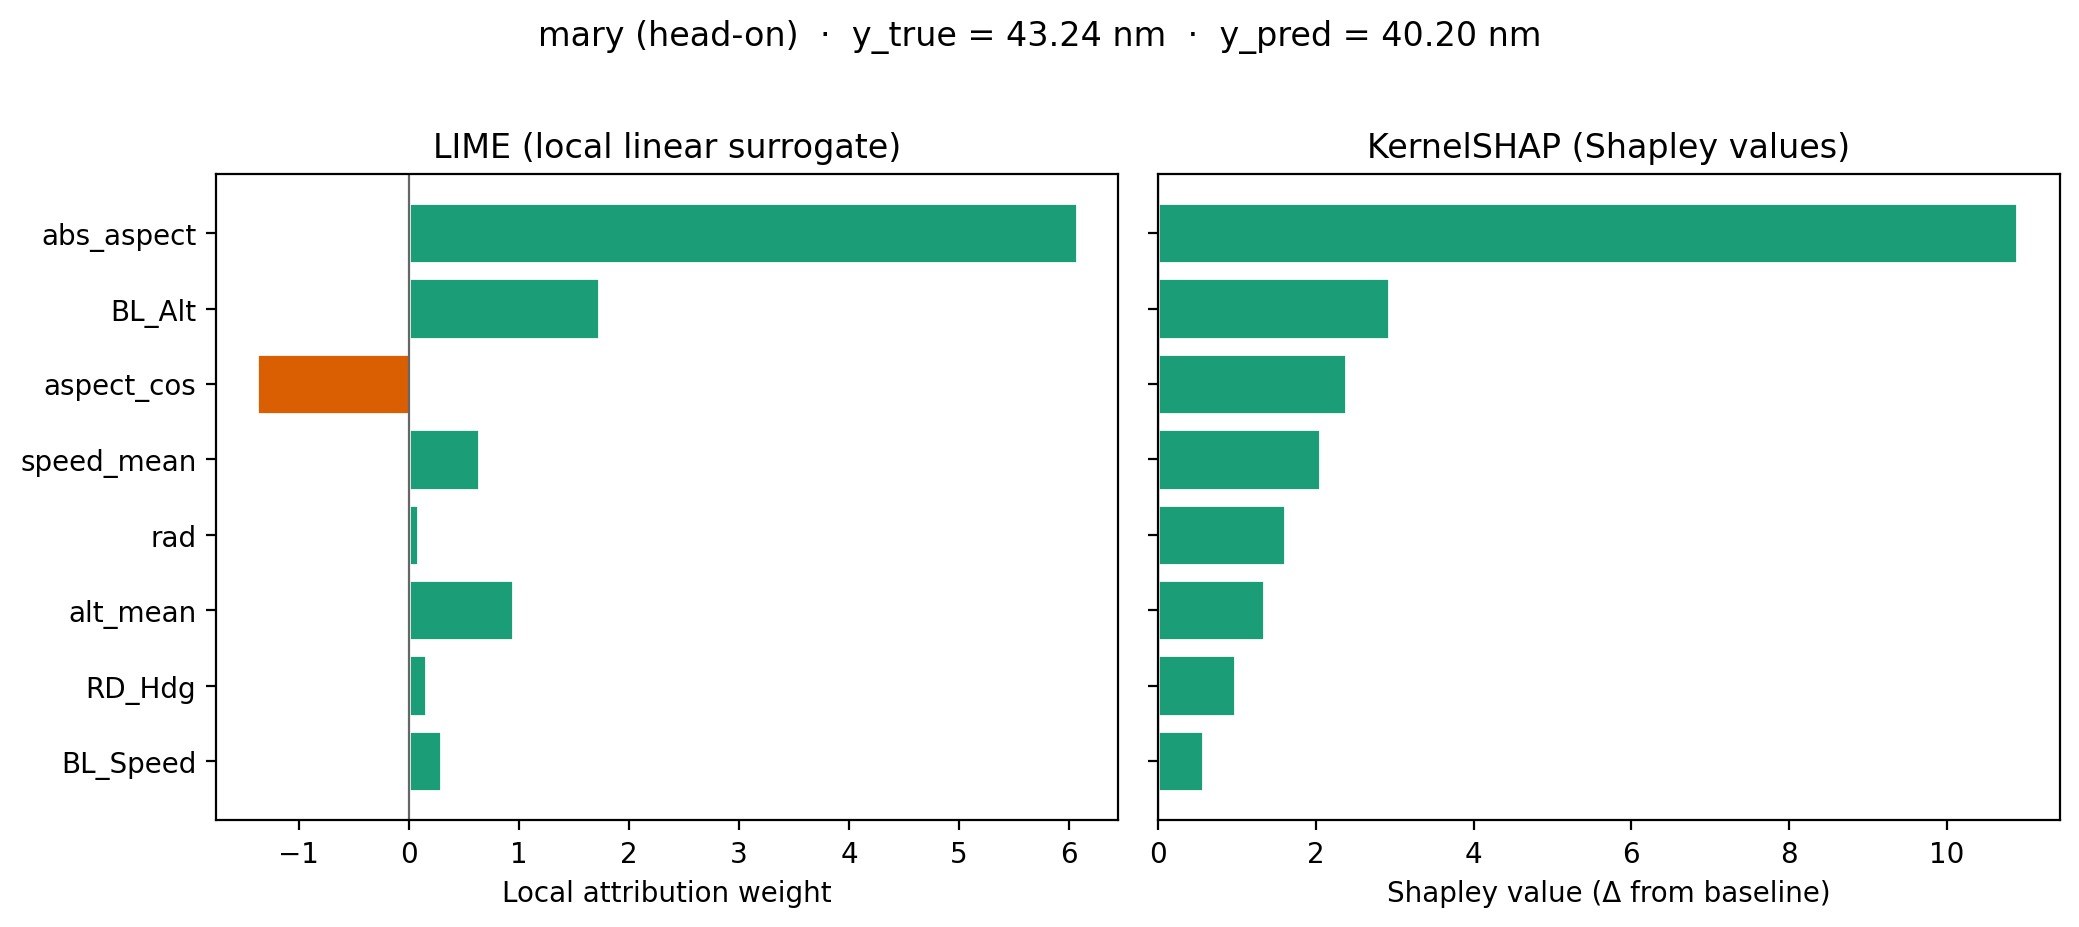
\includegraphics[width=\linewidth]{figs/fig03_mary.png}
\caption{Head-on Mary: LIME (left) vs.\ KernelSHAP (right). Both methods pick $|\alpha|$ as the top contributor. SHAP's attribution magnitude ($10.95$\,nm) is about $1.8\times$ the LIME weight ($6.07$\,nm); the gap matches Shapley's coalition-based accounting, which redistributes more credit to the dominant feature.}
\label{fig:mary}
\end{figure}

\begin{figure}[t]
\centering
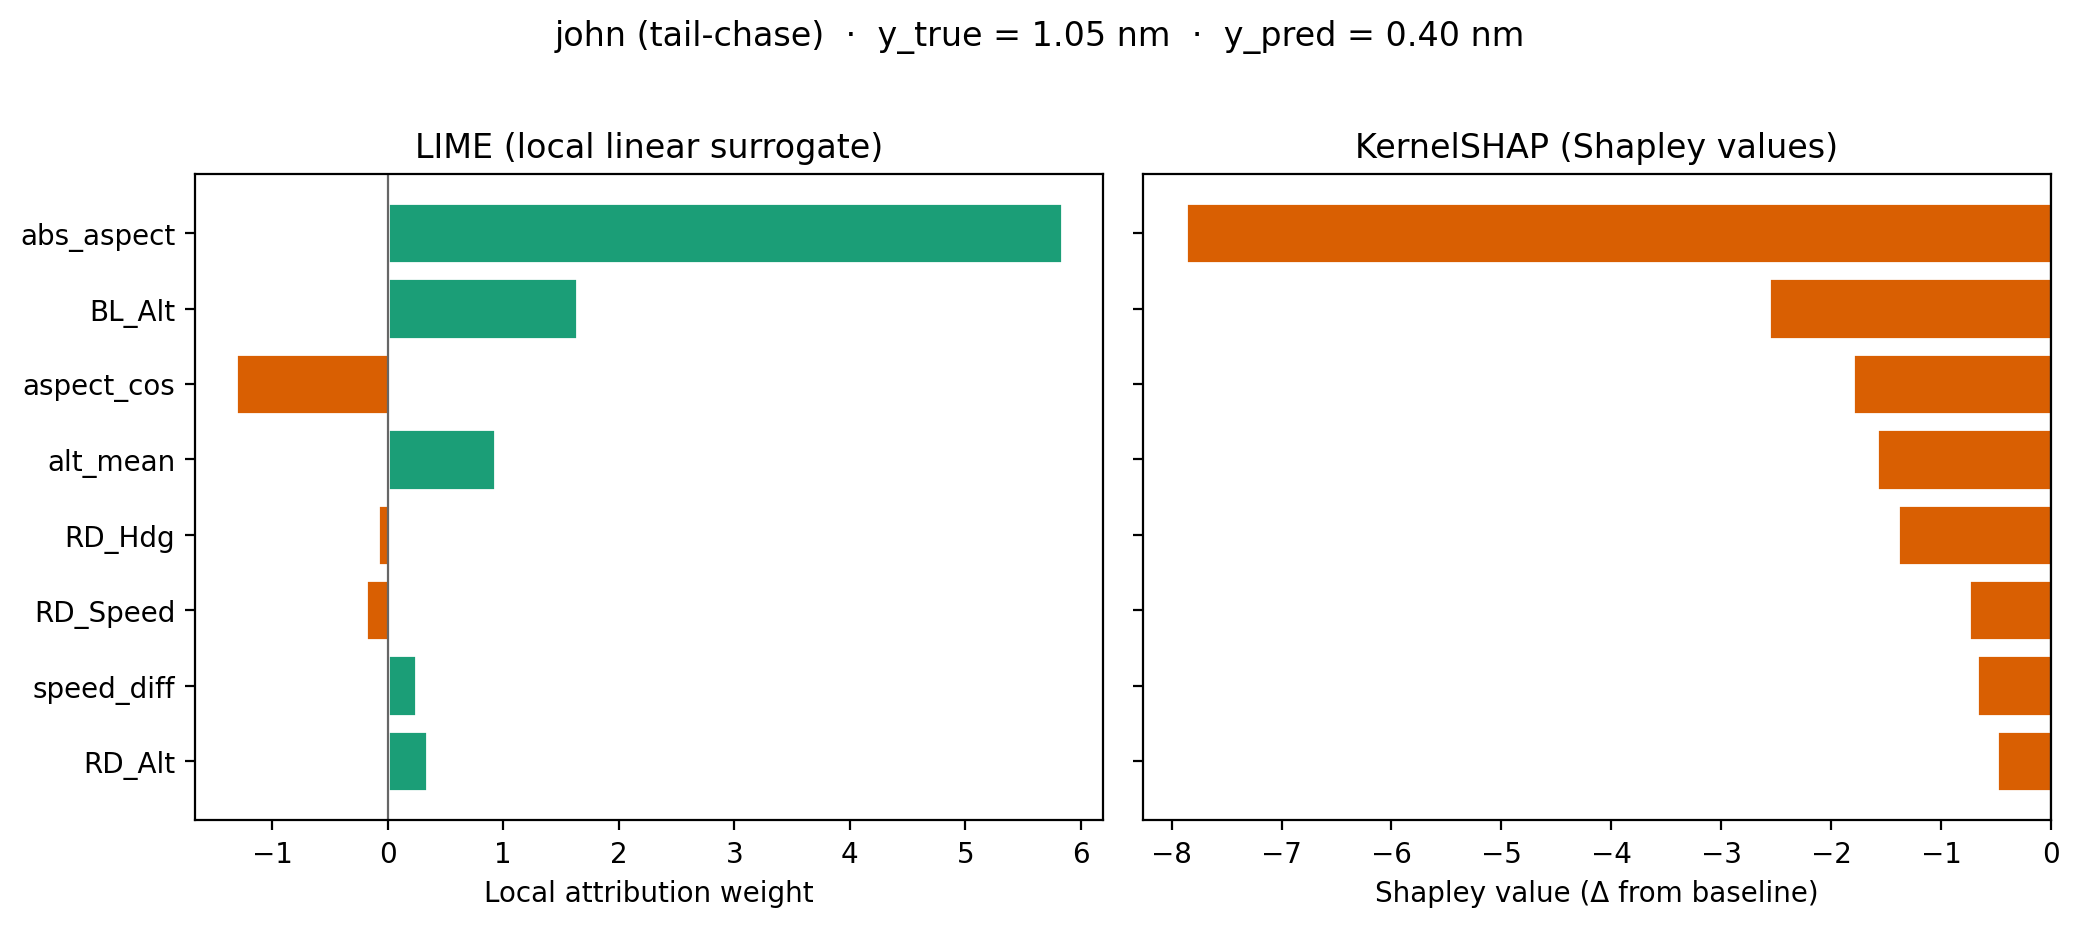
\includegraphics[width=\linewidth]{figs/fig03_john.png}
\caption{Tail-chase John: low altitude, low aspect; both methods correctly attribute the small range to the geometry.}
\label{fig:john}
\end{figure}

\begin{figure}[t]
\centering
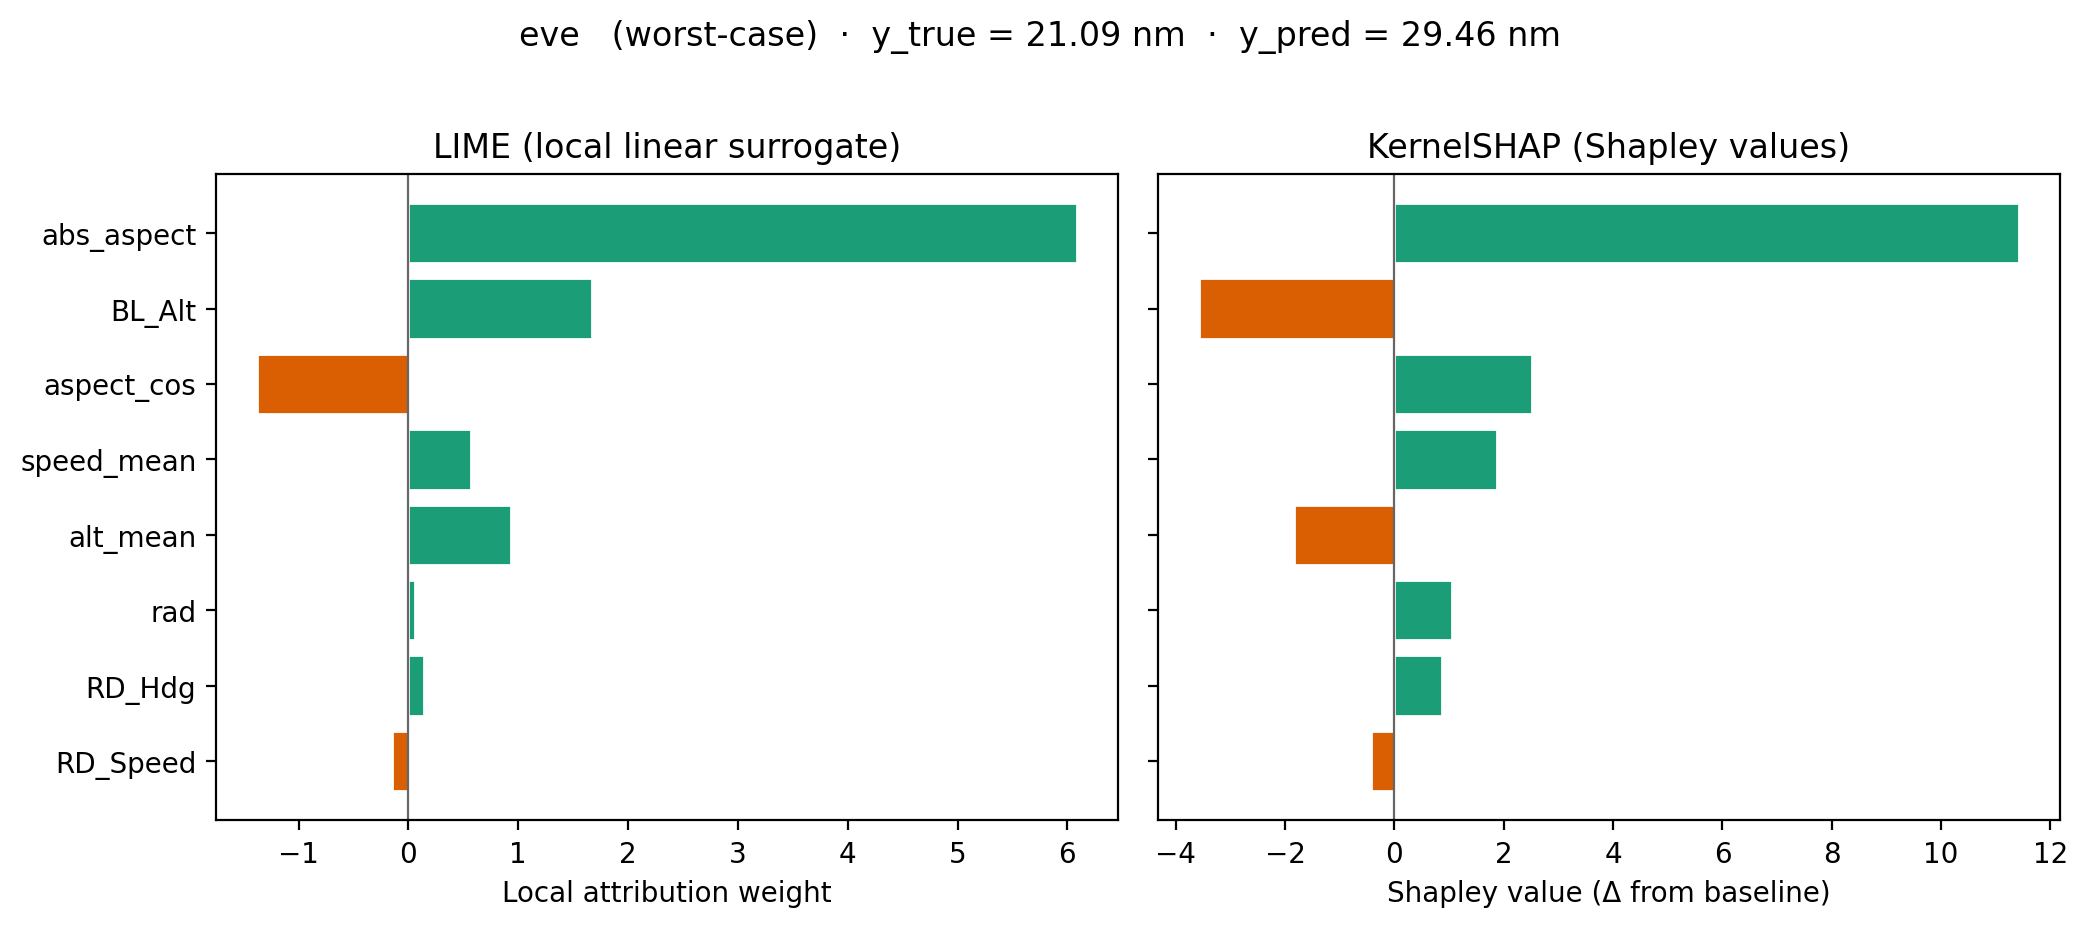
\includegraphics[width=\linewidth]{figs/fig03_eve.png}
\caption{Worst-case Eve: largest absolute error on the OOD set ($|y-\hat{y}|=8.37$\,nm). Both methods agree on $|\alpha|$ as the top feature, but the model structurally over-predicts in this high-energy head-on corner.}
\label{fig:eve}
\end{figure}

\begin{table}[t]
\centering
\caption{Local-XAI summary for fixed archetypes.}
\label{tab:local}
\small
\begin{tabular}{lrrrr}
\toprule
Archetype & $y$ & $\hat{y}$ & $\rho_{\text{top-3}}$ & $\rho_{\text{top-5}}$ \\
\midrule
Mary (head-on)    & 43.24 & 40.20 & 1.00 & 0.83 \\
John (tail-chase) &  1.05 &  0.40 & 1.00 & 0.94 \\
Eve (worst-case)  & 21.09 & 29.46 & 1.00 & 0.90 \\
\bottomrule
\end{tabular}
\end{table}

\subsection{Global explanations (ALE, mean-$|$SHAP$|$, PDP vs.\ ALE)}
Figure~\ref{fig:shap_bar} aggregates SHAP values across the OOD set: $|\alpha|$ dominates ($\overline{|\phi|}=4.88$\,nm), followed by $BL_{\text{Alt}}$ ($1.92$), $\cos\alpha$ ($1.14$), and $\overline{Alt}$ ($1.02$). The dominance of $|\alpha|$ matches the engineered-feature correlation finding. The practical reading is that engagement geometry is the primary driver of $RMax$ prediction, with altitude and speed acting as secondary modifiers rather than independent dominant factors.

Figure~\ref{fig:ale} reports ALE curves for the top-6 features. $|\alpha|$ is monotonically increasing in $\textit{RMax}$ through the head-on regime, which lines up with classical missile pole geometry. The $BL_{\text{Alt}}$ panel is also positive and monotone, the same feature that PDP will misrepresent below.

Figure~\ref{fig:pdp_vs_ale} contrasts PDP and ALE for $BL_{\text{Alt}}$. The PDP curve is biased downward in the upper-altitude regime because it marginalizes over $RD_{\text{Alt}}$ as if it were independent, but $\mathrm{corr}(BL_{\text{Alt}}, RD_{\text{Alt}})=0.97$; the implied joint mass at \textit{high BL, low RD} is almost absent in the data. The ALE estimate, which avoids this extrapolation, is monotone increasing as physics requires. This figure is the concrete reason ALE rather than PDP is reported elsewhere in the paper, and it justifies the methodological choice empirically rather than only on theoretical grounds.

\begin{figure}[t]
\centering
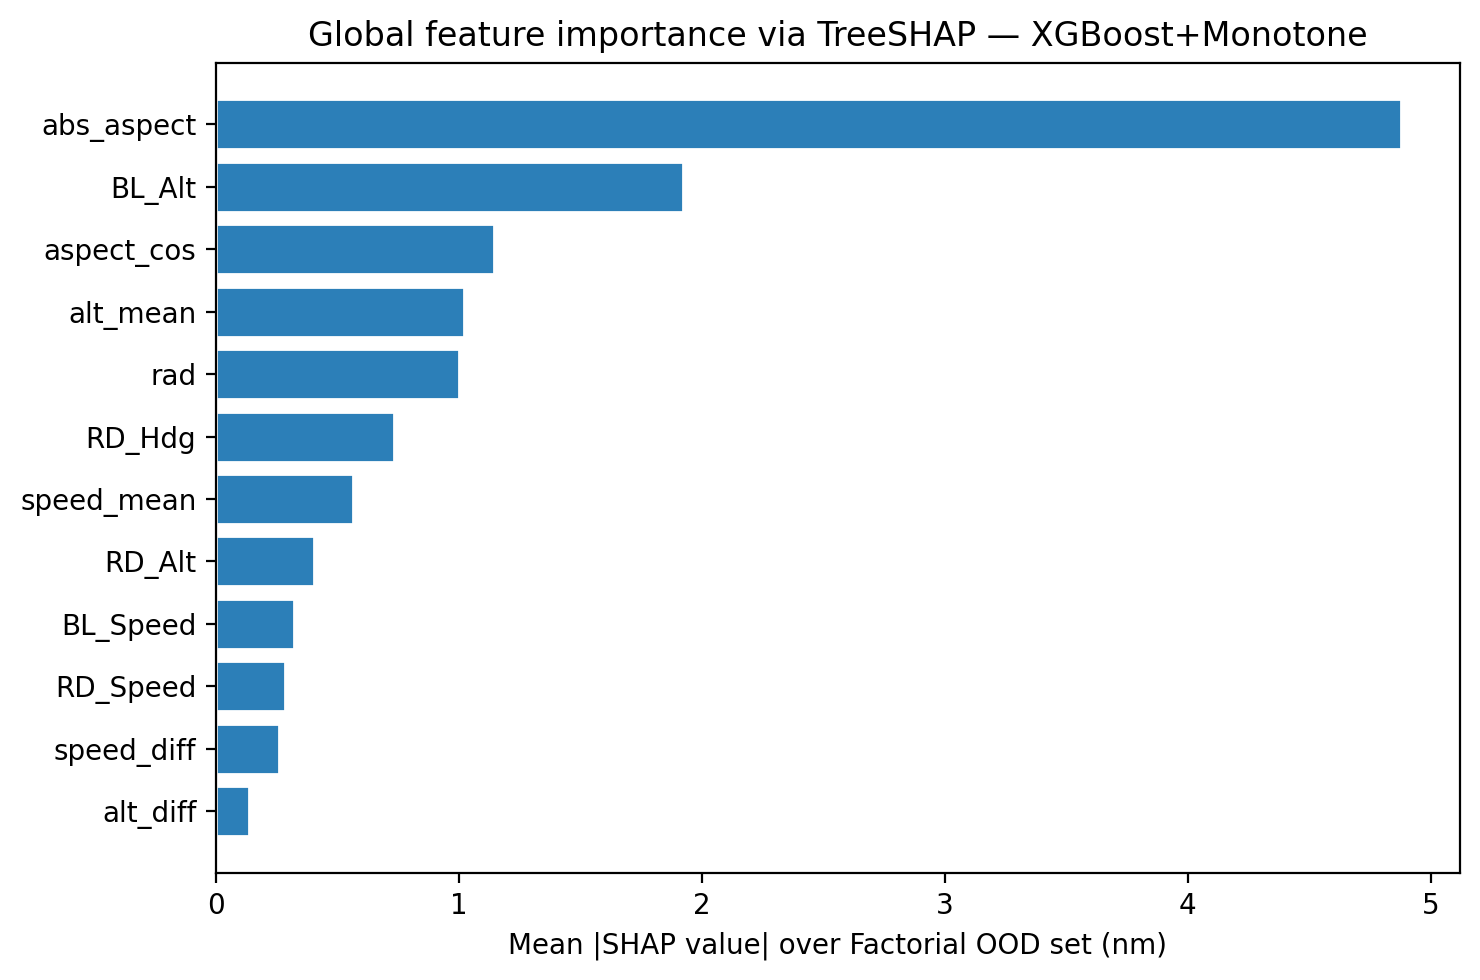
\includegraphics[width=\linewidth]{figs/fig04_global_shap_bar.png}
\caption{Mean $|$TreeSHAP$|$ over the OOD set. $|\alpha|$ alone ($4.88$\,nm) exceeds the sum of the next three features ($4.07$\,nm).}
\label{fig:shap_bar}
\end{figure}

\begin{figure}[t]
\centering
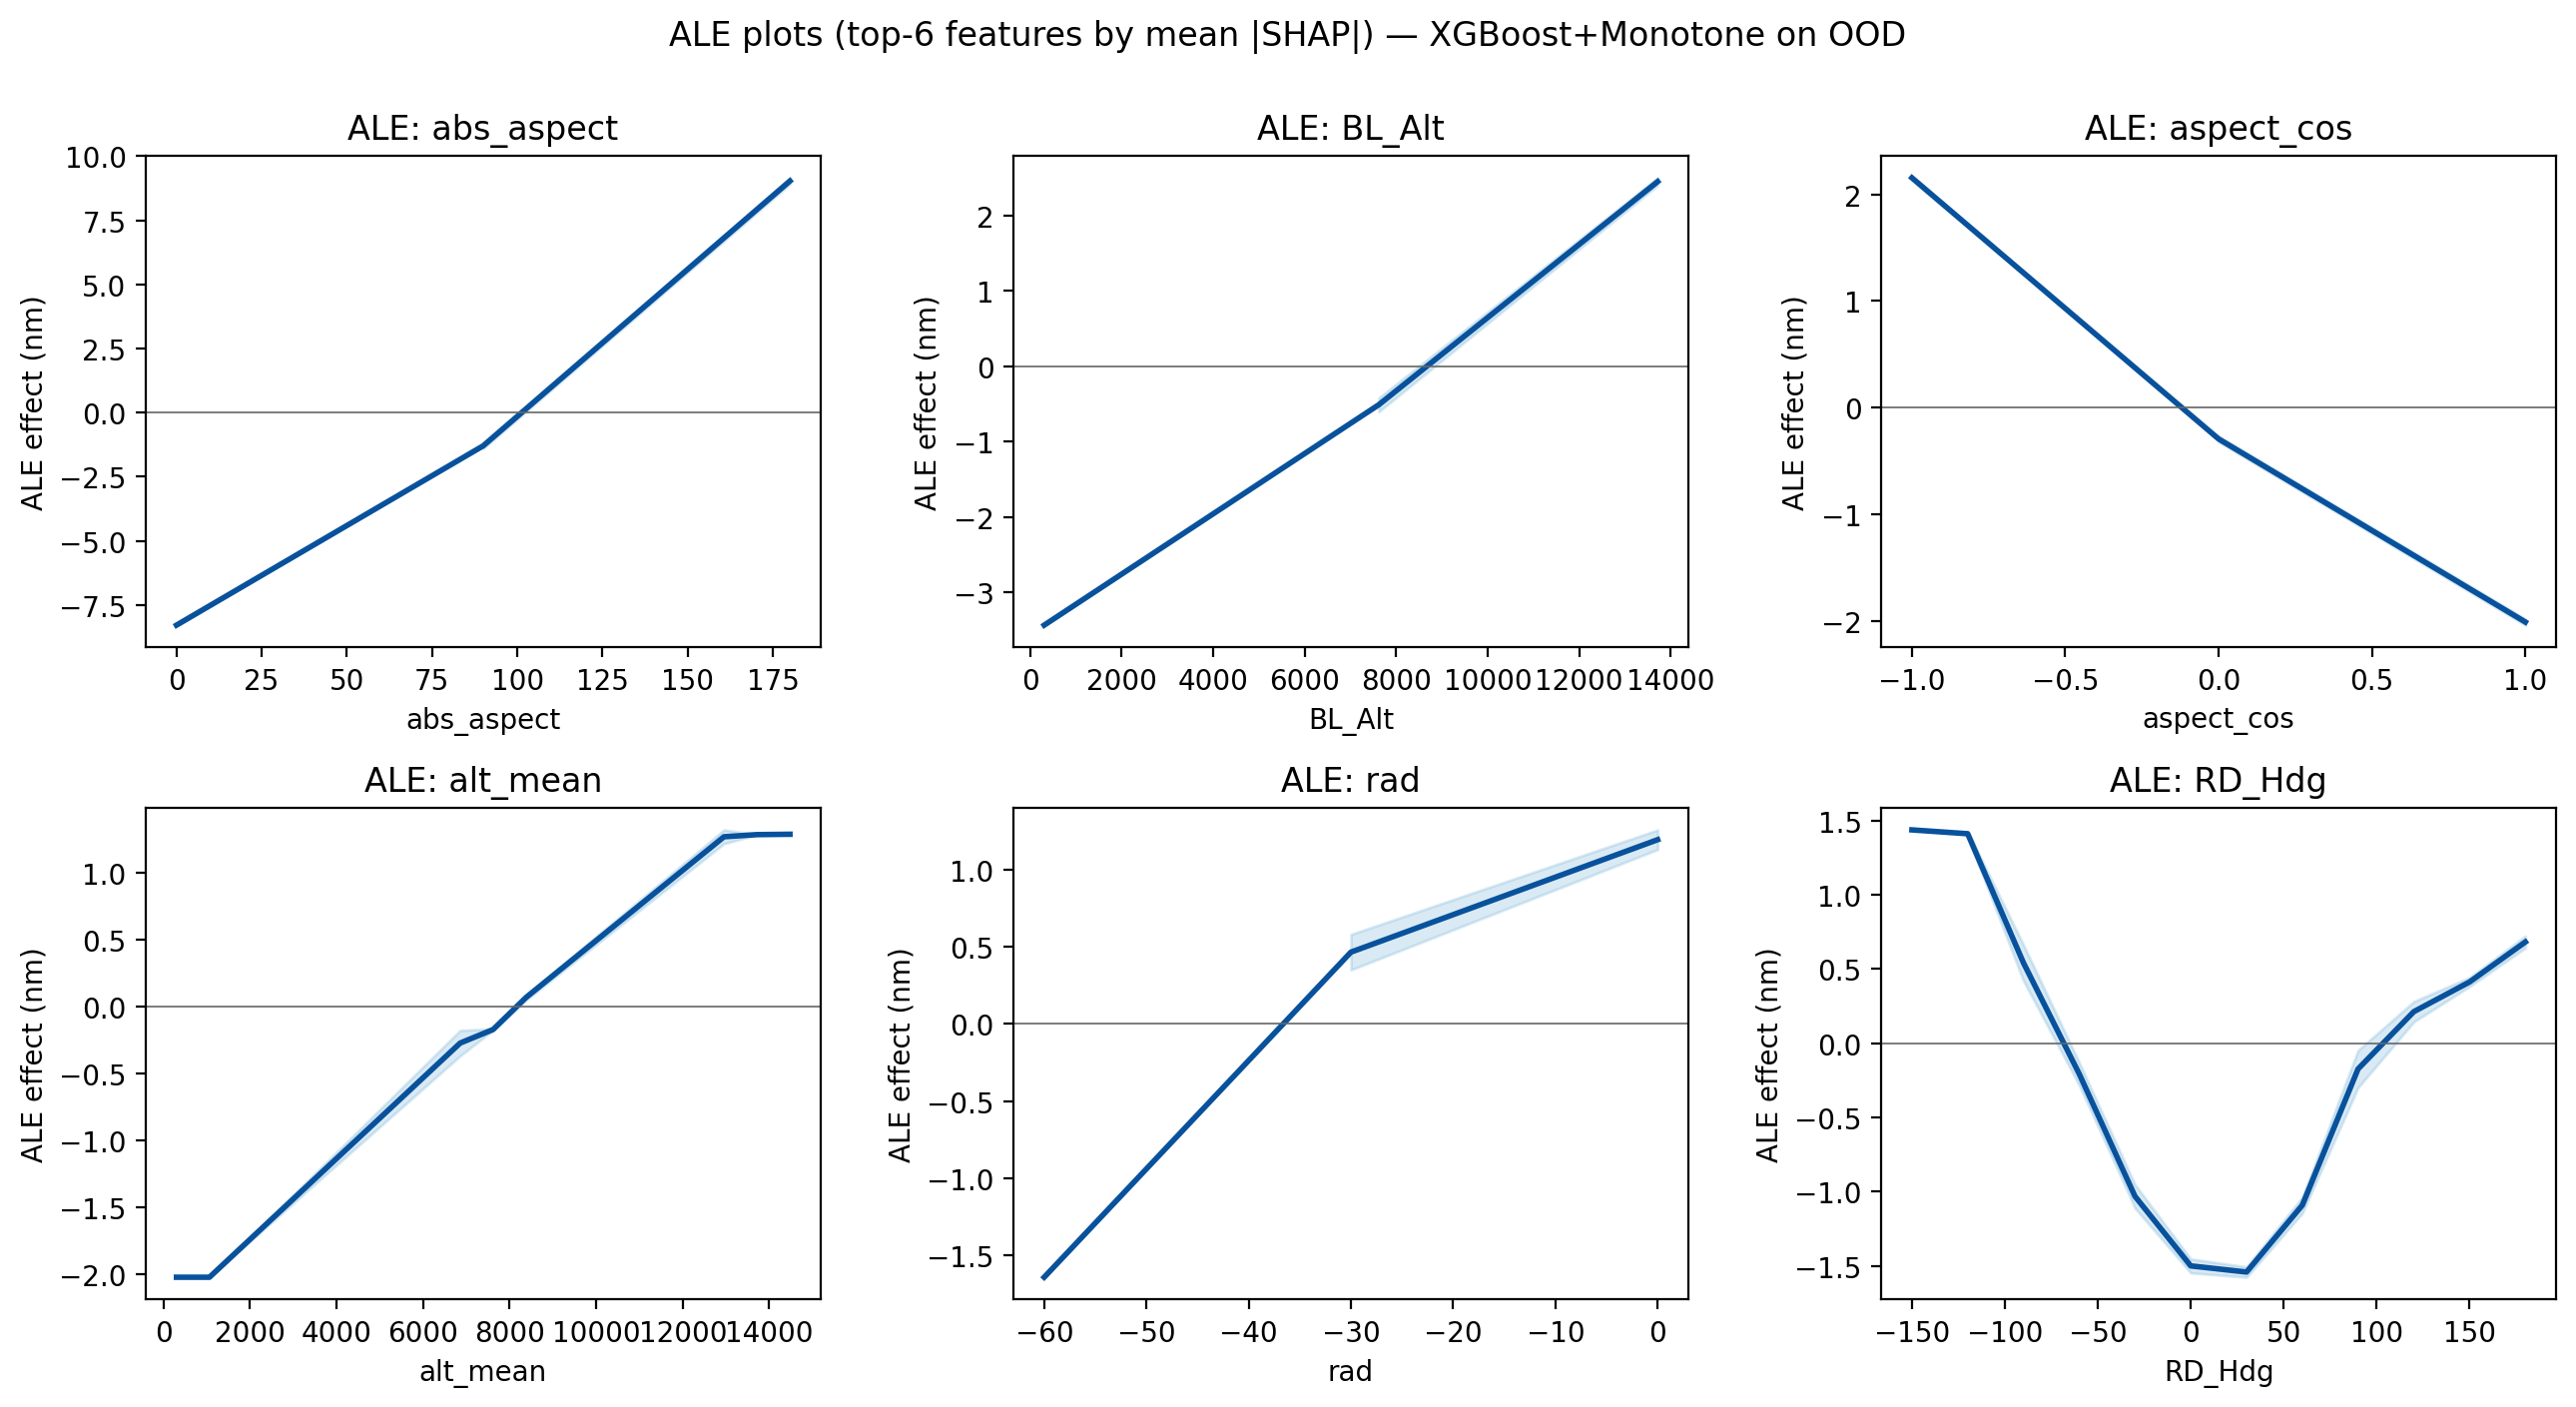
\includegraphics[width=\linewidth]{figs/fig05_ale_top6.png}
\caption{ALE for the top-6 features by mean $|$SHAP$|$. Each curve is the accumulated local effect computed on 20-bin partition of the OOD set.}
\label{fig:ale}
\end{figure}

\begin{figure}[t]
\centering
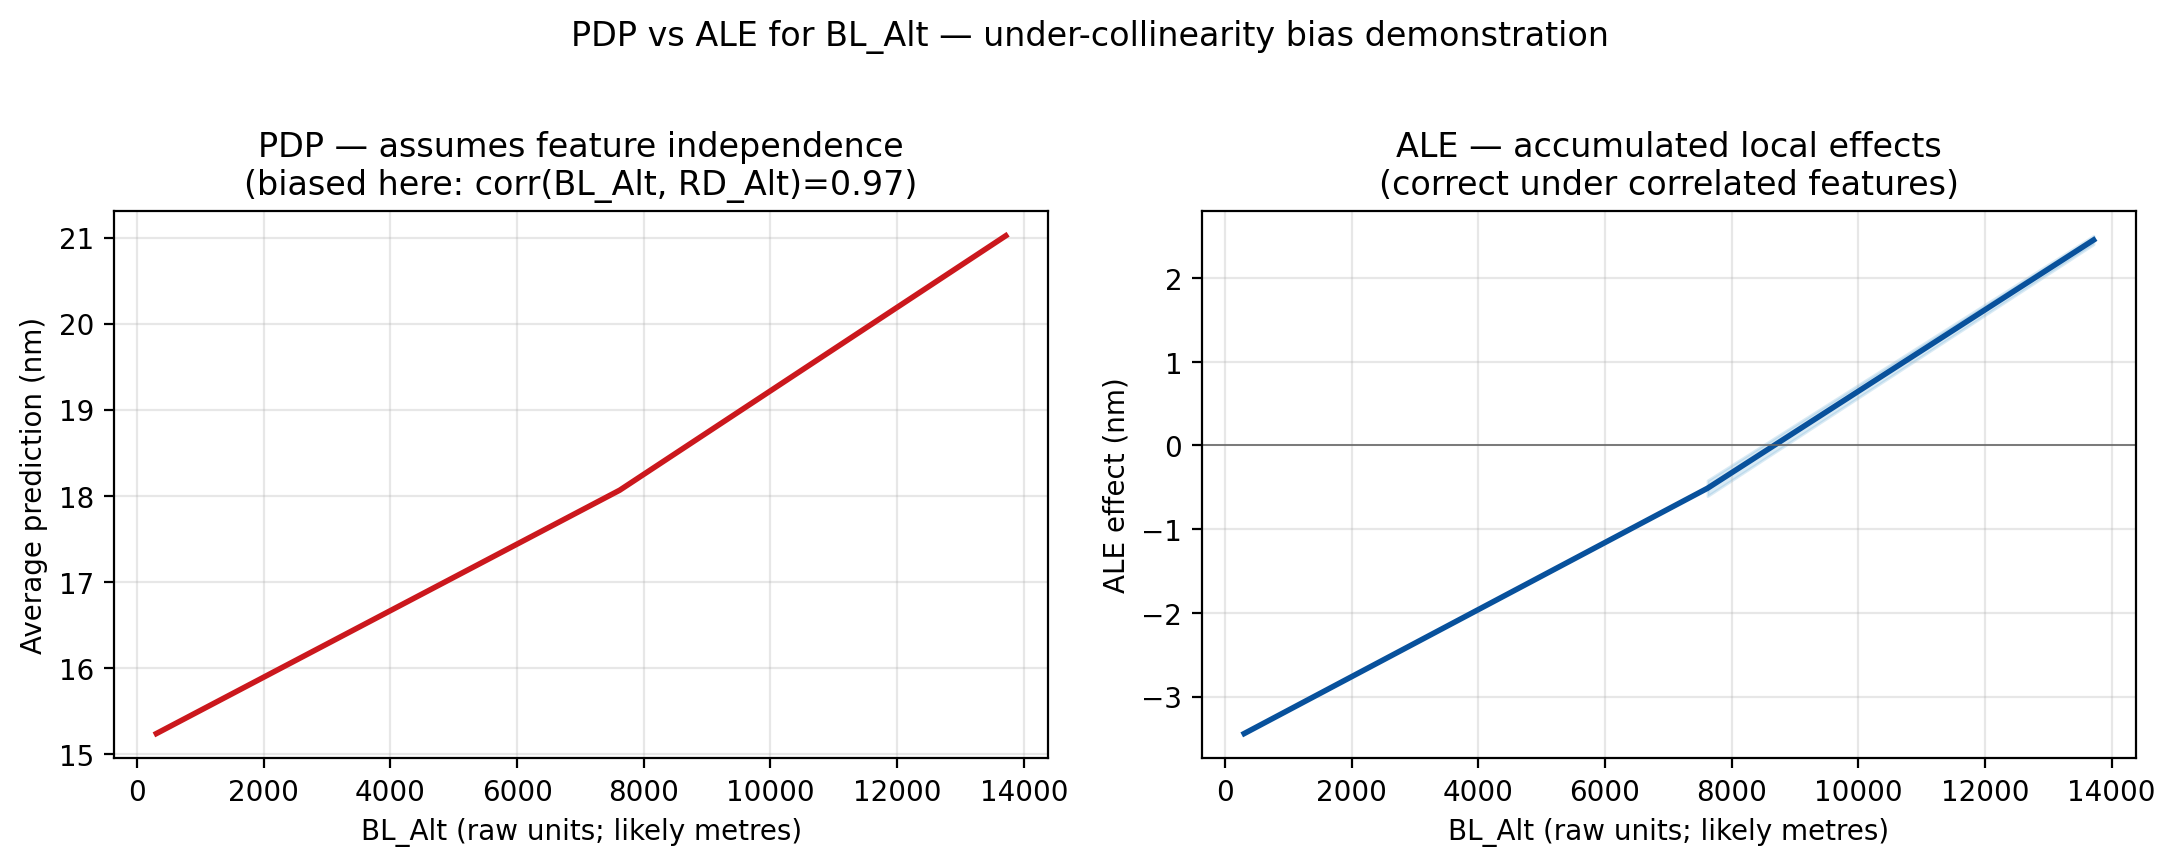
\includegraphics[width=\linewidth]{figs/fig06_pdp_vs_ale_BL_Alt.png}
\caption{PDP (left) vs.\ ALE (right) for $BL_{\text{Alt}}$. Under the $BL_{\text{Alt}}$-$RD_{\text{Alt}}$ collinearity ($r=0.97$), PDP is biased; ALE is monotonically increasing as physics predicts.}
\label{fig:pdp_vs_ale}
\end{figure}

\subsection{Model-specific: monotone ablation and physics audit}
The model-specific component plays a double role: it provides interpretation and at the same time improves the model. Monotone constraints inject physics priors directly into the XGBoost splits, reducing OOD MAE from $1.177$\,nm (unconstrained) to $1.101$\,nm. The paired-bootstrap test on per-instance absolute errors gives
\begin{equation*}
    \Delta\text{MAE}_{\text{mono-vs-XGB}} = -0.076\;\text{nm},\;\; \text{CI}_{95} = [-0.13, -0.02],
\end{equation*}
i.e., the constraints lower OOD MAE by a small but statistically significant $0.08$\,nm. The in-distribution effect is in the same direction ($-0.06$\,nm CV MAE), so the constraints improve both regimes rather than trading one against the other.

The explanation half of the same contribution comes from the TreeSHAP interaction values (Figure~\ref{fig:inter}): the three largest off-diagonal cells are $(|\alpha|, \overline{V})=0.21$\,nm, $(\rho, |\alpha|)=0.14$\,nm, and $(|\alpha|, BL_{\text{Alt}})=0.10$\,nm. All three involve $|\alpha|$ as one leg and a kinematic or altitude term as the other; these interactions are consistent with the aspect-speed and aspect-altitude couplings expected from WEZ geometry. Table~\ref{tab:physics} closes the loop with the physics-consistency audit: 6/6 audited features have SHAP-correlation signs matching the prior, all at $|\rho|>0.90$. Figure~\ref{fig:audit} visualizes the audit. The single model-specific component therefore plays two roles at once: it improves performance through monotone constraints and explains the source of the improvement through interaction values.

\begin{table}[t]
\centering
\caption{Physics-consistency audit. All six audited features pass.}
\label{tab:physics}
\small
\begin{tabular}{lcrc}
\toprule
Feature & Expected & Spearman & Pass \\
\midrule
$|\alpha|$           & $+$ & $+0.908$ & \checkmark \\
$\cos\alpha$         & $-$ & $-0.908$ & \checkmark \\
$BL_{\text{Alt}}$    & $+$ & $+0.934$ & \checkmark \\
$\overline{Alt}$     & $+$ & $+0.958$ & \checkmark \\
$BL_{\text{Speed}}$  & $+$ & $+0.943$ & \checkmark \\
$RD_{\text{Speed}}$  & $-$ & $-0.943$ & \checkmark \\
\bottomrule
\end{tabular}
\end{table}

\begin{figure}[t]
\centering
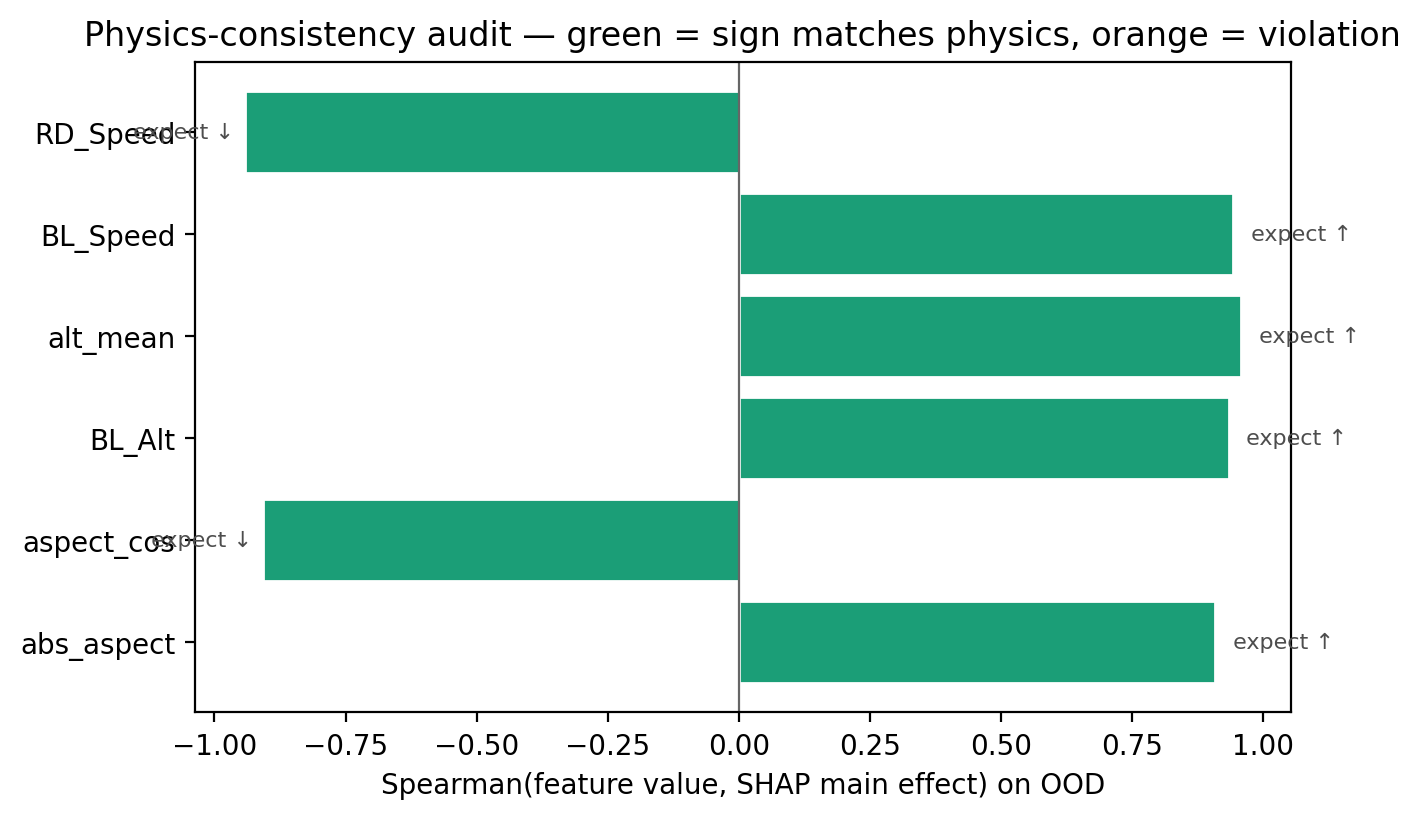
\includegraphics[width=\linewidth]{figs/fig09_physics_audit.png}
\caption{Physics-consistency audit. Green = sign matches physics. All six audited features pass.}
\label{fig:audit}
\end{figure}

\begin{figure}[t]
\centering
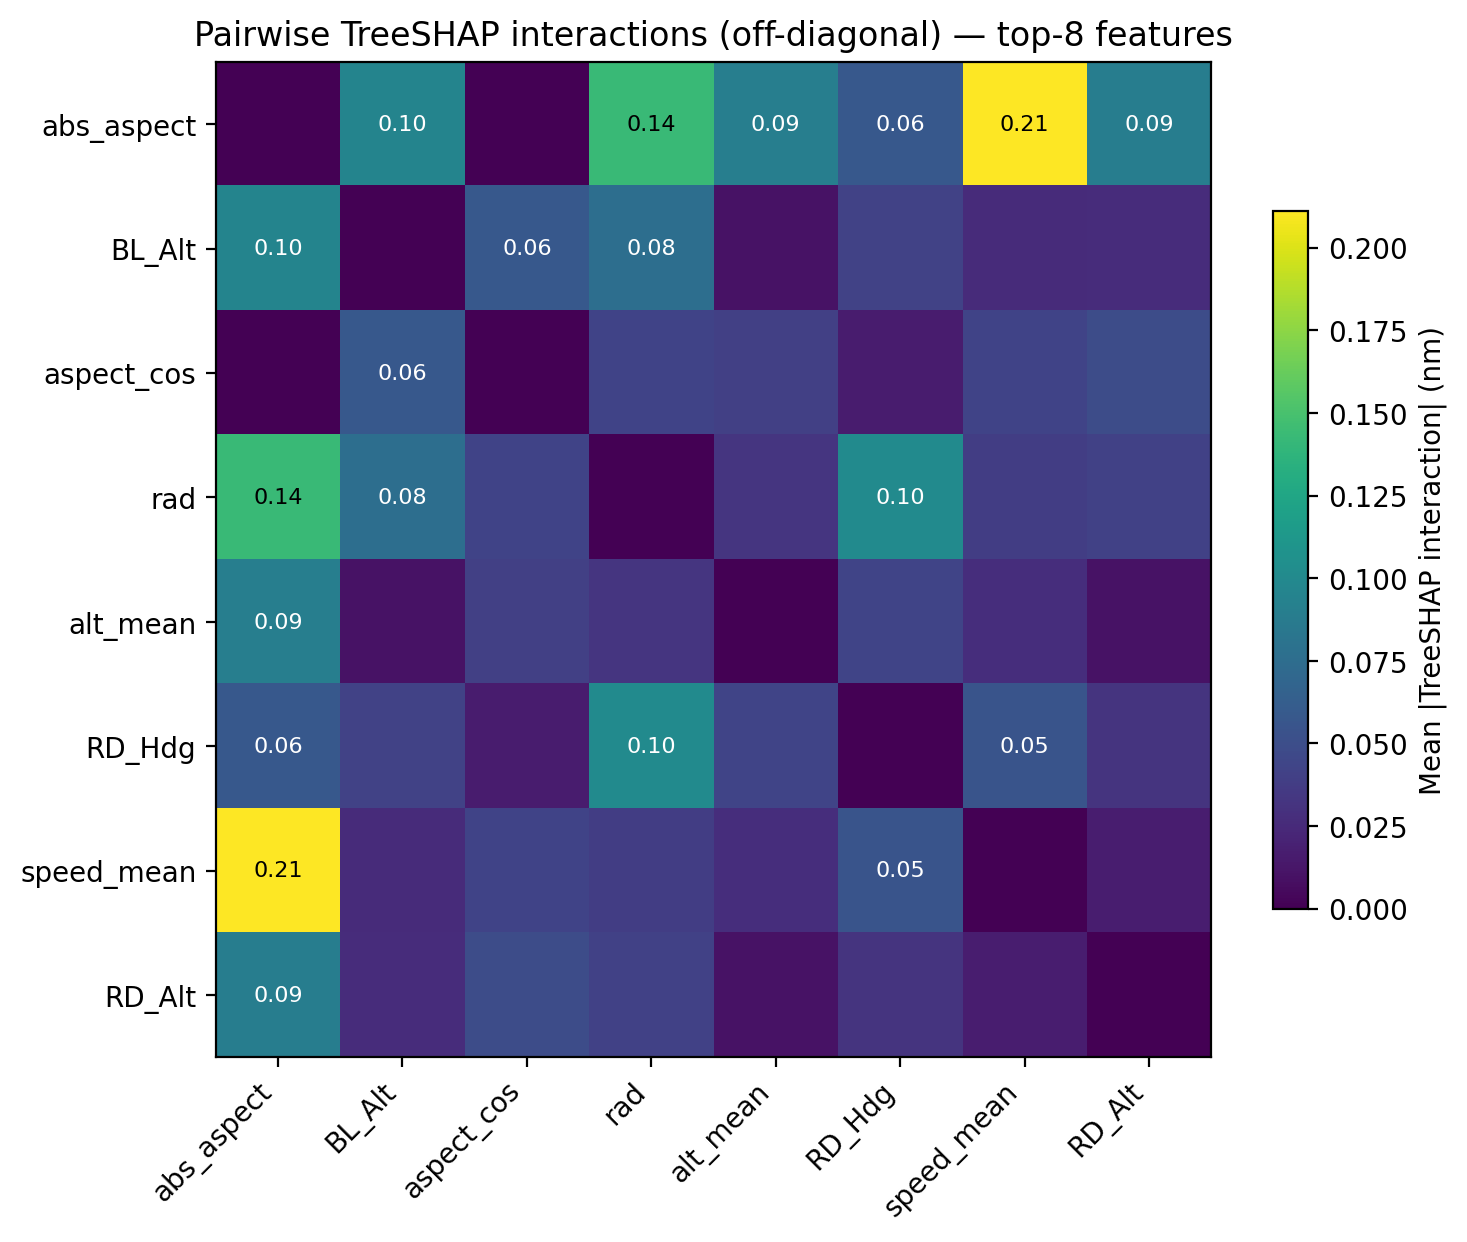
\includegraphics[width=\linewidth]{figs/fig07_treeshap_interactions.png}
\caption{Pairwise TreeSHAP interaction matrix (off-diagonal, top-8 features). The three largest off-diagonal cells are $(|\alpha|, \overline{V})=0.21$, $(\rho, |\alpha|)=0.14$, and $(|\alpha|, BL_{\text{Alt}})=0.10$; all three involve $|\alpha|$ as one leg, which says aspect dominates as a main effect and again as the partner in pairwise couplings.}
\label{fig:inter}
\end{figure}

\subsection{Disagreement across the OOD set}
We scan $N=80$ randomly selected OOD instances and compute the top-3 Spearman LIME--SHAP rank-agreement (Figure~\ref{fig:disagree}). Top-1 attribution still agrees on every archetype, but the deeper ranks disagree often: median top-3 $\rho = -0.10$, with $70\%$ of instances below $\rho = 0.5$. The Spearman correlation between rank-agreement and absolute prediction error is essentially zero ($+0.02$), so disagreement does not track model difficulty in this dataset. On this corpus, LIME--SHAP disagreement on the secondary ranks is therefore best interpreted as attribution variability rather than as a per-instance uncertainty signal; the methods agree on the dominant aspect feature and diverge elsewhere roughly independently of the prediction error. This still matches Krishna et al.~\cite{krishna2022} qualitatively, in that the two methods are not redundant; it does not, on this dataset, provide a reliable per-instance score.

\begin{figure}[t]
\centering
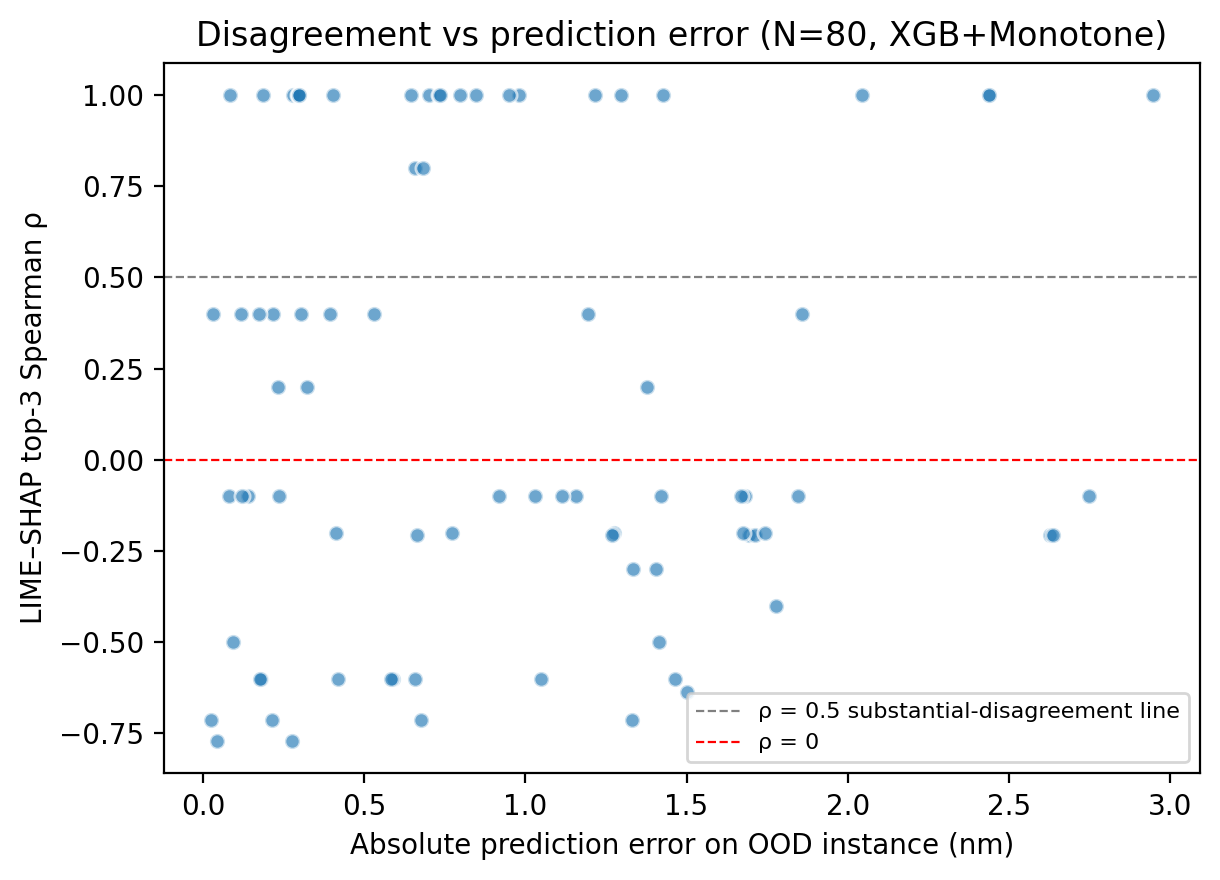
\includegraphics[width=\linewidth]{figs/fig08_disagreement_vs_error.png}
\caption{LIME--SHAP top-3 rank-agreement vs.\ absolute OOD error across 80 sampled instances. The cluster spans the full $[-1, 1]$ range with no monotone trend against error.}
\label{fig:disagree}
\end{figure}

\subsection{Conformal intervals}
Split-conformal calibration with $\alpha=0.10$ on a 30\%-holdout calibration set of Random gives a residual quantile $q=1.74$\,nm and an interval width of $3.48$\,nm. On a within-distribution test set the bands reach the nominal $90\%$ by construction; on the held-out Factorial OOD set empirical coverage settles at $67.1\%$ (Figure~\ref{fig:conformal}). The under-coverage is the expected behavior when calibration and test distributions differ; it is also informative, since the gap between nominal and empirical coverage on Factorial directly quantifies how OOD the Factorial set really is. A practical fix is split-conformal calibrated on a small Factorial holdout, which we leave to future work to avoid burning OOD samples; locally adaptive variants (Mondrian, weighted) are another option in the same direction.

\begin{figure}[t]
\centering
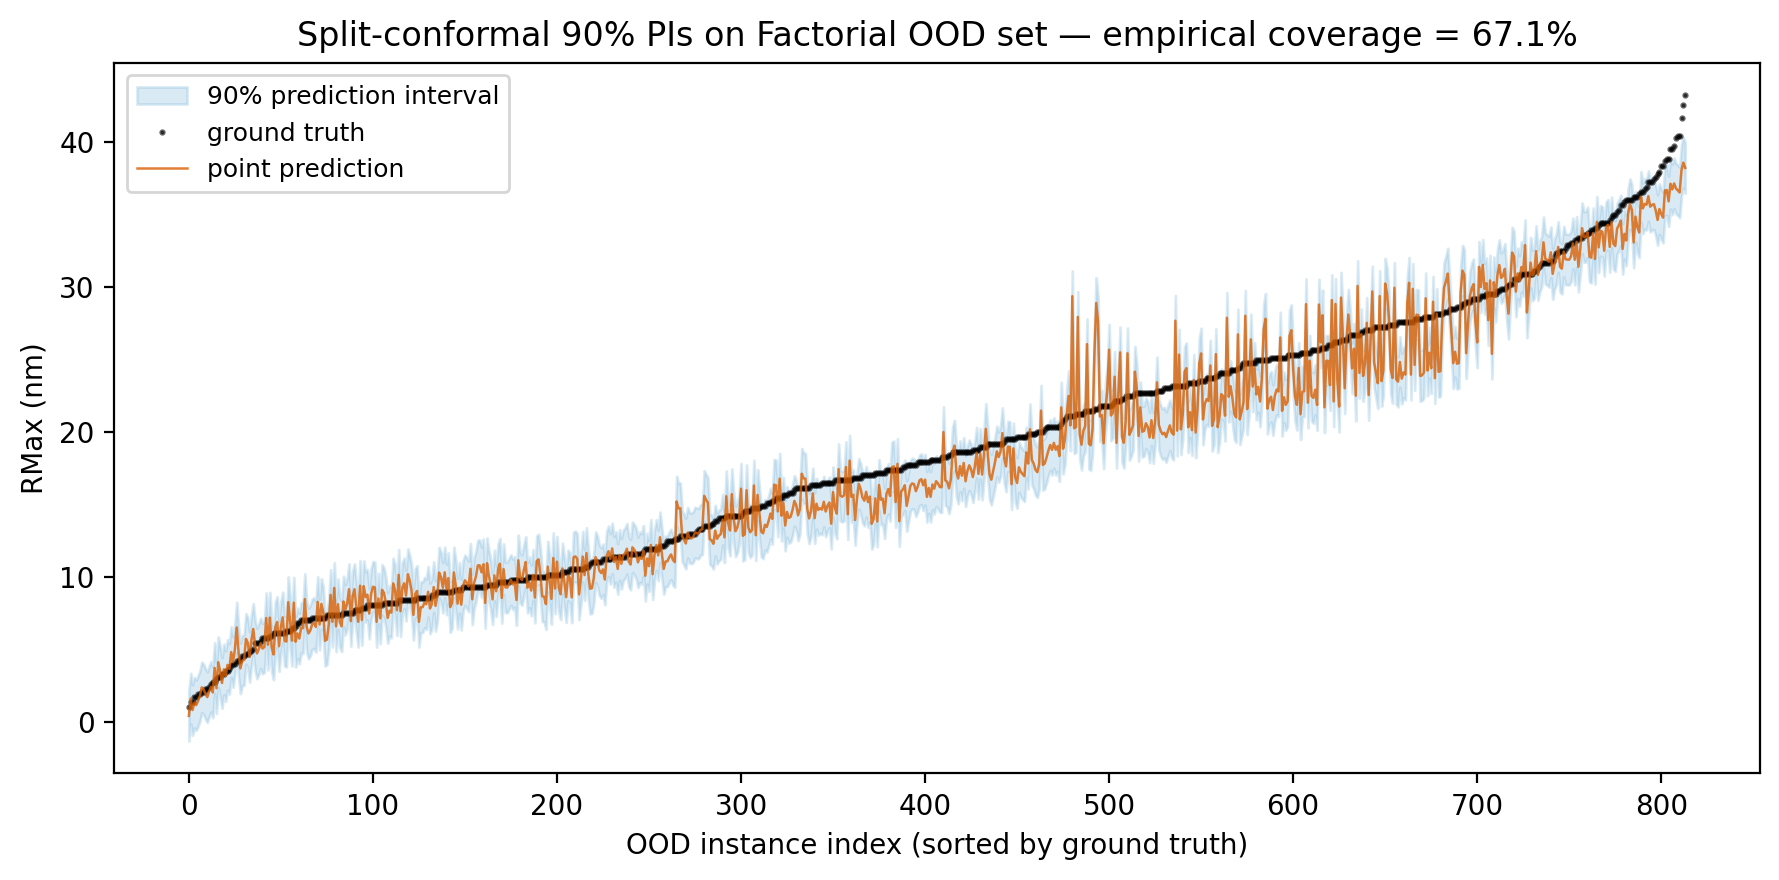
\includegraphics[width=\linewidth]{figs/fig11_conformal.png}
\caption{Split-conformal nominal-$90\%$ intervals on the Factorial OOD set. Empirical coverage $=67.1\%$ at mean width $3.48$\,nm; the under-coverage exposes residual distribution shift between Random calibration and Factorial OOD.}
\label{fig:conformal}
\end{figure}

\subsection{Symmetry sanity check}
Simultaneous sign-flip of $(\rho, RD_{\text{Hdg}})$ leaves the engagement geometry invariant; an idealized model should produce identical predictions. Figure~\ref{fig:sym} shows that the XGBoost+Monotone model is only \emph{approximately} symmetric: predictions cluster on the diagonal but with a measurable scatter. Quantitatively, mean signed difference is $-0.29$\,nm, standard deviation is $0.73$\,nm, $44.7\%$ of OOD instances fall within $0.5$\,nm of perfect invariance, and max $|\text{diff}|$ reaches $2.51$\,nm. The residual asymmetry is a real model failure mode: the Random training sweep covers $\rho \in [-60^{\circ}, +60^{\circ}]$ but is not perfectly balanced across the sign axis, and the model has absorbed that handedness via the $\sin\alpha$ feature. This residual asymmetry is also diagnostically useful, since the model's own symmetry residual flags inputs the geometry alone cannot disambiguate. The natural fix is a symmetry-augmented training pass that mirrors each Random sample about the sign axis; we leave this to future work.

\begin{figure}[t]
\centering
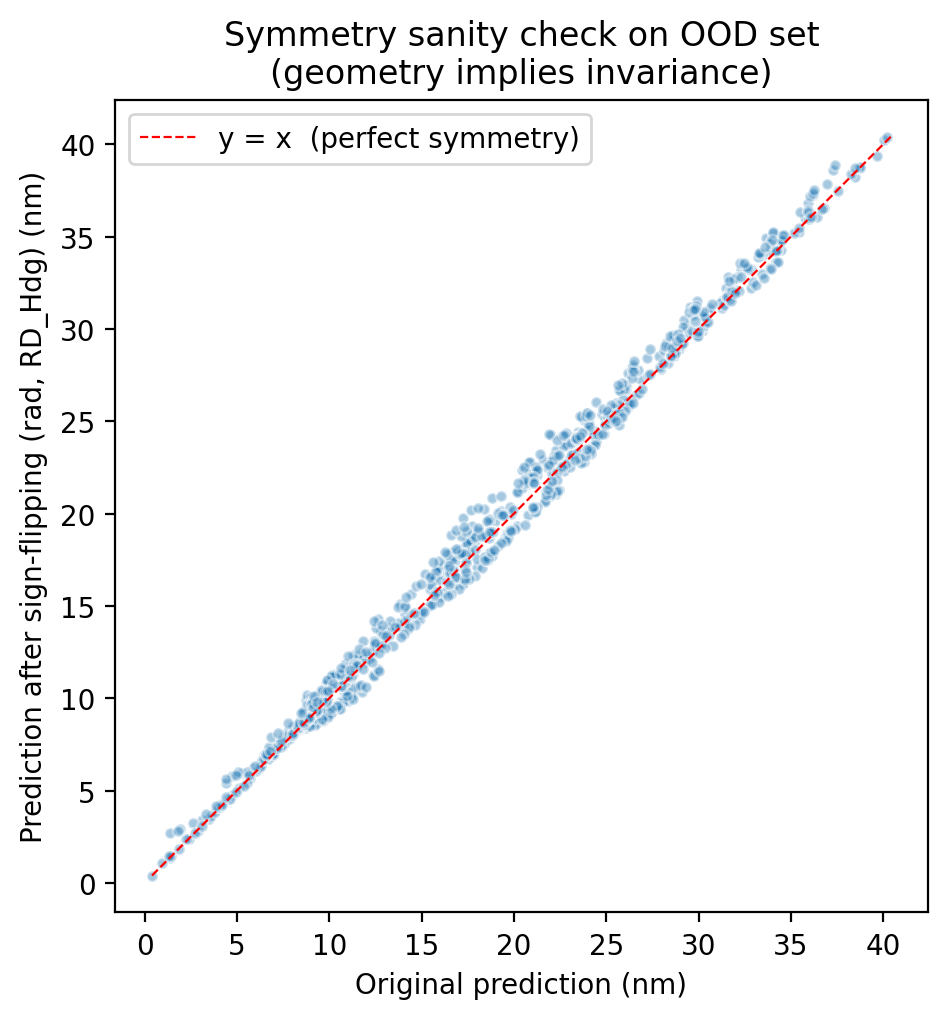
\includegraphics[width=\linewidth]{figs/fig10_symmetry.png}
\caption{Predictions before vs.\ after simultaneous sign-flip of $(\rho, RD_{\text{Hdg}})$. Points cluster around the diagonal but with measurable scatter (std $0.73$\,nm, max $|\text{diff}|$ $2.51$\,nm); the geometric invariance is only approximately respected.}
\label{fig:sym}
\end{figure}

\subsection{Multi-output portability: RNez}
We swap the target column from \textit{RMax} to \textit{RNez} and re-run the entire pipeline without any other change. The Factorial CSV does not carry \textit{RNez}, so we report $5\times 5$ repeated stratified CV on Random (Table~\ref{tab:rnez}). All three model classes generalize without code change. The narrower \textit{RNez} dynamic range ($1.05$--$17.93$\,nm vs.\ \textit{RMax}'s $1.93$--$39.02$) shrinks the absolute MAE proportionally; the ordering across models is preserved, with monotone-XGBoost retaining the edge ($0.378$\,nm).

\begin{table}[t]
\centering
\caption{Multi-output portability: same pipeline, swap target. CV on Random, no Factorial OOD because the Factorial CSV omits \textit{RNez}.}
\label{tab:rnez}
\scriptsize
\setlength{\tabcolsep}{4pt}
\begin{tabular}{lrrrr}
\toprule
                  & \multicolumn{2}{c}{RMax ($n{=}964$)} & \multicolumn{2}{c}{RNez ($n{=}923$)} \\
\cmidrule(lr){2-3}\cmidrule(lr){4-5}
Model             & CV MAE & CV $R^2$ & CV MAE & CV $R^2$ \\
\midrule
EBM (GA$^2$M)        & 0.864 & 0.985 & 0.405 & 0.957 \\
XGBoost              & 0.828 & 0.986 & 0.408 & 0.953 \\
XGBoost + Monotone   & \textbf{0.765} & \textbf{0.989} & \textbf{0.378} & \textbf{0.960} \\
\bottomrule
\end{tabular}
\end{table}

\subsection{Stage-0 feasibility classifier}
\label{subsec:stage0}
The Random sweep contains $36$ infeasible rows ($3.6\%$ base rate). At this imbalance, AUROC and AUPRC against the feasible-as-positive convention are uninformative (the majority class is at $96.4\%$ already, so AUPRC saturates near $1$); the operationally relevant numbers are computed against the \emph{infeasible}-as-positive convention, reported in Table~\ref{tab:stage0}.

The two classifiers behave very differently at the default decision threshold. LogReg with balanced class weights catches $94\%$ of infeasibles (the operationally critical task) but only $26\%$ of its infeasible flags are correct, with $101$ false alarms on the feasible side across the 5 folds. EBM-Classifier reverses the trade-off: only $39\%$ infeasible recall, but $93\%$ precision and only $2$ false alarms. For a WEZ overlay that should prefer flagging a borderline engagement to silently accepting an infeasible one, the LogReg operating point is the safer choice; the EBM variant suits a setting where false alarms are expensive and a missed infeasibility can be caught downstream by the conformal interval. Both classifiers expose $1 - \Pr[\textit{feasible}\mid\mathbf{x}]$ as an input-side uncertainty score, complementary to the output-side conformal width.

\begin{table}[t]
\centering
\caption{Stage-0 feasibility metrics (5-fold stratified CV on full Random table). AUROC and AUPRC are computed with \emph{infeasible} as the positive class. CM cells are aggregated across folds, rows = true, cols = predicted.}
\label{tab:stage0}
\scriptsize
\setlength{\tabcolsep}{4pt}
\begin{tabular}{lrrrrr}
\toprule
Classifier & AUROC$_{\text{inf}}$ & AUPRC$_{\text{inf}}$ & Recall & Precision & F1 \\
\midrule
LogReg          & 0.964 & 0.484 & \textbf{0.943} & 0.261 & 0.406 \\
EBM-Classifier  & \textbf{0.986} & \textbf{0.790} & 0.393 & \textbf{0.933} & \textbf{0.526} \\
\bottomrule
\addlinespace[2pt]
\multicolumn{6}{l}{\textbf{Aggregated confusion matrices} (rows = [infeas, feas], cols = pred):} \\
\multicolumn{6}{l}{\quad LogReg: $[[34,\,2],\,[101,\,863]]$;\quad EBM-Clf: $[[14,\,22],\,[2,\,962]]$} \\
\bottomrule
\end{tabular}
\end{table}

% =================================================================
\section{Discussion}
\label{sec:discussion}
% =================================================================

\subsection{Interpretable vs.\ Black-Box Performance}
The OOD MAE gap between EBM ($1.754$\,nm) and monotone-XGBoost ($1.101$\,nm) is $0.65$\,nm, with monotone-XGBoost giving the strongest predictive performance on this corpus. The Hit@2nm gap is also substantial: EBM reaches $63.6\%$ and both XGBoost variants reach $84.5$--$84.6\%$. The operational target ($\Pr[\,|f - RMax| < 2\,\text{nm}\,] \geq 0.80$) is therefore met by the XGBoost variants but not by EBM. For a fielded WEZ overlay, EBM's microsecond-latency shape-function inspection is attractive, but its operating point is below the operational target. The recommendation depends on whether the pilot can absorb the $\sim 20$-point Hit-rate gap in exchange for the explanation latency; on this corpus the gap is large enough to favor monotone-XGBoost as the default and EBM as the auditing companion.

\subsection{Comparison of Local Model-Agnostic Explanations}
Top-1 attributions from LIME and KernelSHAP agree on every archetype, so for the easy explanation question (``which feature mattered most?'') the two methods are interchangeable. Below the top, the picture is noisier: $70\%$ of OOD instances have top-3 rank-agreement $\rho < 0.5$, and the Spearman correlation between rank-agreement and absolute error is essentially zero ($+0.02$). LIME and SHAP do disagree about the secondary feature ranks, but the disagreement does \emph{not} track prediction difficulty. The two methods are not interchangeable below the top, but their disagreement is not by itself a usable per-instance uncertainty score; a Stage-0 feasibility probability and the conformal width remain the more reliable signals.

\subsection{Local vs.\ Global Explanations}
Local SHAP explains a single decision; global ALE describes the model's policy across the input space. They serve different consumers (the pilot wants the first, the systems engineer wants the second), and a report that uses only one is incomplete. The Mary--John--Eve archetypes illustrate the gap. Mary and John are well inside the model's competence and either explanation will do; Eve lies in a high-energy head-on corner where the model structurally over-predicts \textit{RMax}, with local attributions pointing in the right direction but the absolute prediction off by $8.37$\,nm. Global ALE alone would have hidden this failure mode by averaging over the entire OOD set; the local trio is what surfaces it.

\subsection{Model-Specific Interpretation and Improvement}
The model-specific component is required by the rubric to both improve performance and provide an insight. The monotone-XGBoost variant does the first: $-0.08$\,nm OOD MAE relative to unconstrained XGBoost (95\% CI excludes zero) and $-0.06$\,nm in CV; the gap is small but reproducible. TreeSHAP interactions do the second: the three largest pairwise interactions all involve $|\alpha|$, with $(|\alpha|, \overline{V})$ leading at $0.21$\,nm and $(\rho, |\alpha|)$ at $0.14$\,nm. The ablation in Table~\ref{tab:ablation} shows that the dominant gain over a raw-input baseline comes from the engineered aspect feature itself ($1.86 \to 1.18$\,nm OOD MAE); the constraints add a smaller but statistically significant edge on top. The improve-and-explain components are therefore one integrated contribution.

\subsection{Operational Implication and Remaining Failure Modes}
A WEZ overlay built from monotone-XGBoost plus ALE plus conformal intervals meets the operational threshold (Hit@2nm $=84.6\%$ against the $80\%$ target), passes the 6/6 physics audit, and reports its own miscalibration on the genuinely OOD slice ($67.1\%$ empirical against $90\%$ nominal coverage). The symmetry residual in Figure~\ref{fig:sym} gives an additional signal: instances where the geometry-flipped prediction disagrees with the original are flagged for human review. Stage-0 routing covers the feasibility side, while the DiCE counterfactuals (Appendix~\ref{app:dice}) probe the worst-case head-on corner that produces the largest residual error. The most plausible next steps for closing the remaining error are symmetry-augmented training (to reduce the $44.7\%$-within-$0.5$-nm symmetry residual) and a larger Factorial-style sweep for proper OOD calibration of the conformal intervals.

\subsection{Limitations}
The $n=964$ Random sample is small for a six-input regression, and the dataset comes from a single simulator (B-ACE) with no real flight-test cross-check. The Factorial OOD set is interpolation-OOD: full input vectors are off-grid, but every marginal lies inside the Random support. Extrapolation-OOD (engagements beyond the trained altitude or speed band) remains untested. The symmetry violation documented in Section~\ref{sec:results}-H softens the ``physics-guided'' claim of the title to a quantitative one: the audit and the constraints work, but the model still carries a measurable handedness from the training distribution. The DiCE appendix exposes a counterfactual-search artifact in which engineered features drift from the values implied by the raw inputs; the appropriate follow-up is to generate counterfactuals in raw input space and recompute engineered features deterministically. The Stage-0 classifier numbers in Table~\ref{tab:stage0} suggest a deployment-time decision (LogReg's high recall vs.\ EBM's high precision) rather than a single best choice; threshold tuning to the specific operational cost is left for the integrator.

% =================================================================
\section{Conclusion}
\label{sec:conclusion}
% =================================================================
On the public Kuroswiski 2024 WEZ corpus we built an XAI pipeline that (i) audits the data, exposing six previously-unreported integrity findings; (ii) selects EBM and monotone-constrained XGBoost as inherently-interpretable and constrained-black-box candidates; (iii) explains predictions locally (LIME and KernelSHAP) and globally (ALE and mean-$|$SHAP$|$); (iv) quantifies LIME--KernelSHAP disagreement on the OOD set and finds, on this corpus, that it does not by itself track prediction difficulty; (v) couples monotone constraints with TreeSHAP interactions as a single physics-aware contribution; and (vi) audits split-conformal intervals against the OOD set, surfacing a coverage gap that quantifies residual distribution shift. With the LOS-relative aspect feature in place, monotone-XGBoost meets the $80\%$ Hit@2nm operational target ($84.6\%$ on Factorial). The same code-base processes \textit{RNez} without methodological change, showing multi-output portability. The complete project repository is available at \url{https://github.com/firatbozkaya/wez-xai}.

\appendices

\section{Counterfactual for Worst-case Eve}
\label{app:dice}
The worst-case instance is Factorial row $89$, with $y = 21.09$\,nm against $\hat{y} = 29.46$\,nm, an $8.37$\,nm over-prediction. Eve already sits well inside $[10, 30]$\,nm on the prediction side, so the DiCE search was set to find the smallest perturbation that keeps $\hat{y}$ inside that band. The three returned counterfactuals all set $\rho = 0$ and $|\alpha| = 180^{\circ}$ (head-on geometry) at altitude $\sim 305$\,m, with speeds in $\{(750, 750), (750, 657), (750, 750)\}$\,kn for $(BL_{\text{Speed}}, RD_{\text{Speed}})$, with one of the three swapping $RD_{\text{Alt}}$ up to $\sim 10$\,km. The resulting predictions land in $\{29, 30, 29\}$\,nm. The pattern is consistent with the physics audit: head-on geometry, high own speed, and high altitude push the prediction toward the upper end of the operational band. The Eve over-prediction itself is therefore a structural feature of how the model treats high-energy head-on engagements rather than a local instability. As noted in Section~\ref{sec:discussion}-F, the DiCE optimizer treats raw and engineered features as independent inputs, which can produce counterfactuals whose engineered fields drift from the values implied by the raw inputs; running DiCE in raw input space with deterministic recomputation of the engineered features is the appropriate fix.

\bibliographystyle{IEEEtran}
\bibliography{refs}

\end{document}
